\chapter{Construcción de las bases de Legendre discretas}
\label{cap 2}

En este capítulo vamos a construir,
para toda dimensión $n \geq 2$,
una base ortonormal de $\IR^{n}$,
que llamaremos ``base de Legendre discreta'',
y que en principio se basa en discretizaciones puntuales
de polinomios de ciertos grados
y ortonormalizaciones de las colecciones
de vectores de $\IR^{n}$ que de esto resulta. 
A lo largo del capítulo 
daremos construcciones alternativas de esta base.

Comenzamos planteando algunas definiciones.

\section{Discretización puntual, polinomios discretos y espacios asociados}
\label{discretizacion puntual, polinomios discretos y espacios asociados}

\begin{marginfigure}
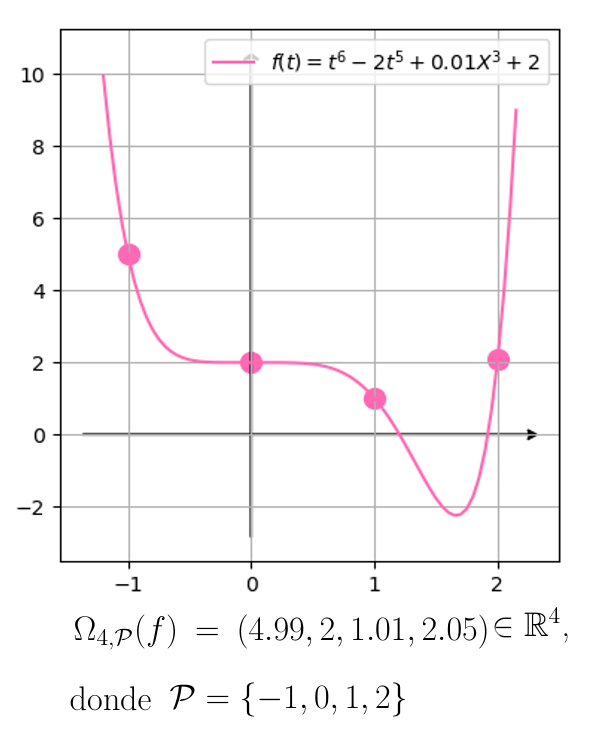
\includegraphics[scale=0.9]{1En_1} 
		\caption{Ejemplo concreto con $n=4$.}
\end{marginfigure}


\begin{defi}
\label{def: operador de discretizacion puntual}
(\textbf{Operador de discretización} $\Omega_{n,\cali{P}}$)
Sea $\cali{P}$ una malla uniforme 
de $n$ puntos
\[
\cali{P}:=\{ t_{j}:=t_{0}+hj : \hspace{0.1cm} 0 \leq j \leq n-1 \},
\]
donde $h \in \IR^{+}$ es una constante fija
(que llamamos el \textbf{paso} de la malla).
Nuestra primera forma de discretizar
a una función $f$ cuyo dominio contenga a los puntos
de la malla $\cali{P}$
consistirá en evaluarla en cada uno de los
puntos de la malla:

\begin{center}
$\Omega_{n,\cali{P}}(f) := (f(t_{j}))_{j=0}^{n-1}.$
\end{center}
\end{defi}


\noindent $\Omega_{n,\cali{P}}$
puede pensarse como una aplicación con dominio
$\cali{C}[t_{0}, t_{n-1}]$,
el espacio de funciones 
continuas en $[t_{0}, t_{n-1}]$,
y con codominio $\IR^{n}$, pero conviene 
identificar al resultado 
de la acción de $\Omega_{n,\cali{P}}$ sobre una
función $f$ con la restricción $f_{| \cali{P}}$
de 
$f$ al conjunto discreto $\cali{P}$,
es decir, con la función

\begin{center}
\aplica{f_{|\cali{P}}}
{\cali{P}}
{\IR }
{t_{j}}{f(t_{j}).}
\end{center}



\begin{defi} \label{def: polinomio discreto}
En el caso en el que $f$ sea elemento de $\IR[t]$, 
nos referiremos
al vector $\Omega_{n,\cali{P}}(f) \in \IR^{n}$
como un \textbf{polinomio discreto de dimensión $n$ con dominio uniforme $\cali{P}$.} 
\end{defi} 

\marginnote{
En lo que sigue, siempre que se hable de un polinomio
discreto
se supondrá que la malla $\cali{P}$
a partir de la que se obtuvo es uniforme.}


Mostraremos en la subsección
\ref{definicion del concepto de grado para seniales finitas}
que, de hecho, \textbf{todo}
$x \in \IR^{n}$ es un polinomio discreto
de dimensión $n$,
y propondremos una definición del grado de este.
Ya podríamos dar algunos resultados en esta dirección,
pero preferimos esperar hasta tener las herramientas
para justificar detalles como la buena definición
de nuestra propuesta de grado (c.f. 
\ref{definicion del concepto de grado para seniales finitas}).


Por la forma en que se definen la suma y la multiplicación
por escalares en los espacios vectoriales $\IR[t]$
y $\IR^{n}$, la siguiente observación es clara.

\begin{obs} \label{obs:linealidad de omega restringida a R[x]}
Sean $n \in \IN$ y $\cali{P}=\{t_{j}:
\hspace{0.2cm}0 \leq j \leq n-1 \}$ una malla uniforme
de $n$ puntos.
La función $\Omega_{n , \cali{P}}$ 
definida en 
\ref{def: operador de discretizacion puntual}
es una transformación lineal de 
$\cali{C}[t_{0}, t_{n-1}]$ a $\IR^{n}$.
\end{obs}
 
El siguiente resultado, que es una consecuencia directa
del Teorema fundamental del álgebra, se usará en repetidas ocasiones.

\begin{prop}
\label{prop: consecuencia del TFA}
Sean $n \geq 2$ y 
$\cali{P}=\{ t_{j}:=t_{0}+hj : \hspace{0.1cm} 0 \leq j \leq n-1 \}$ 
una malla uniforme de $n$ puntos.
Si $f(t) \in \IR[t]$ es un polinomio de grado menor a $n$ y
$\Omega_{n, \cali{P}}(f)$ es el vector cero de $\IR^{n}$, entonces
$f$ es el polinomio cero.
\end{prop}
\noindent
\textbf{Demostración.}
El que $\Omega_{n, \cali{P}}(f)=(f(t_{j}))_{j=0}^{n-1}$ sea
el vector cero significa que los $n$ elementos de la malla
$\cali{P}$ son raíces del polinomio $f$; puesto que, por hipótesis,
$\partial(f) < n$, por la proposición
\ref{prop: cita TFA}
concluimos que
$f$ es el polinomio cero.
\QEDB
\vspace{0.2cm}




\begin{notacion} \label{notacion: Pn, fk, Wi, vk}
Sean $n \in \IN$ y $k$ un entero no negativo.
Denotaremos 
por $\IR_{k}[t]$ al subespacio de $\IR[t]$
que consta de los polinomios de grado a lo más $k$.
\noindent
Escribiremos como $f_{k}$ 
a las potencias básicas,
es decir, a los polinomios
\begin{equation}
\label{fk}
f_{k}(t):=t^{k}.
\end{equation}
Denotaremos por $\cali{P}_{n}$ a la siguiente
malla uniforme:
\begin{equation}
\label{malla Pn}
\cali{P}_{n}=\{ 0, 1, \ldots , n-1 \}.
\end{equation}
A la discretización puntual del
polinomio $f_{k}$ en la malla 
$\cali{P}_{n}$
la denotaremos por $v_{k}$;
\begin{equation}
\label{vectores vk}
v_{k}:= \Omega_{n, \cali{P}_{n}}(f_{k})
=(f_{k}(j))_{j=0}^{n-1}=(j^{k})_{j=0}^{n-1}.
\end{equation}
\end{notacion}

\begin{defi}
\label{def: espacis Wni}
Sean $n\geq 2$ y
$0 \leq i \leq n-1$ enteros.
Definimos al subespacio 
$W_{n,i}$ de $\IR^{n}$ como sigue:
\begin{equation}
\label{espacios Wi}
W_{n,i} := span\{ v_{k} : 0 \leq k \leq i \} \subseteq \IR^{n},
\end{equation}

\noindent
donde los vectores $v_{k}$ son como en \ref{vectores vk}.
\end{defi}


En la ecuación \eqref{espacios Wi} con la que se
define al espacio $W_{n,i}$,
siempre conviene pensar al primer subíndice $n$
como el \textbf{índice de dimensión}, pues corresponde
a la dimensión del espacio ambiente $\IR^{n}$,
y al subíndice $i$ como \textbf{índice de grado};
más adelante (c.f. tercer punto del teorema 
\ref{cor: propiedades importantes de espacios Wi}) 
se verá por qué este es un buen nombre.



\begin{obs} \label{obs:independencia lineal polinomios}
Sea $n \in \IN$. Si $i \in \overline{\IN}$, entonces
los $i+1$ polinomios
$f_{k}$ con $0 \leq k \leq i$ entero
constituyen una base para el espacio $\IR_{i}[t]$.
\end{obs}



\begin{prop} \label{obs: s en Wi sii es la discretizacion en malla Pn de un pol de grado a lo más i}
Sea $n \in \IN$.
Una señal $x=(x_{k})_{k=0}^{n-1}$ de dimensión $n$
es elemento del espacio $W_{n,i}$ 
definido en \eqref{espacios Wi}
si y sólo si 
$x$ es la discretización en $\cali{P}_{n}$
de un polinomio de grado a lo más $i$.
\end{prop}
\noindent
\textbf{Demostración.}
En efecto, según la definición del espacio
$W_{n,i}$ y la linealidad del operador
de discretización 
$\Omega$ establecida en 
la observación
\ref{obs:linealidad de omega restringida a R[x]}, 
tenemos que $x \in \IR^{n}$ es elemento de 
$W_{n,i}$ si y sólo si existen números reales
$a_{k}$ con $0 \leq k \leq i$ tales que
\begin{align*}
x=  \suma{k=0}{i}{a_{k}v_{k}} 
=  \suma{k=0}{i}{a_{k}\Omega_{n, \cali{P}_{n}}(f_{k})}
=  \Omega_{n, \cali{P}_{n}} \left( 
\suma{k=0}{i}{a_{k}f_{k}} \right)
=  \Omega_{n, \cali{P}_{n}} (g),
\end{align*}
con $g := \suma{k=0}{i}{a_{k}f_{k}} \in \IR_{i}[t]$
(c.f. observación 
\ref{obs:independencia lineal polinomios}).
\null\nobreak\hfill\ensuremath{\square} %final dem


De las definiciones de señales constantes, afines
y cuadráticas (c.f. \ref{def: grafica senial})
y la proposición 
\ref{obs: s en Wi sii es la discretizacion en malla Pn de un pol de grado a lo más i}
se sigue de inmediato el siguiente resultado.
\begin{cor} \label{cor: condiciones necesarias y suficientes para que x sea afín en términos de pertenencia a espacios Wi}
Sean $n \in \IN$ y $x \in \IR^{n}$ una señal de dimensión
$n$ cualquiera.
\begin{itemize}
\item La señal $x$ es constante si y sólo si $x \in W_{n,0}$,

\item es afín si y sólo si $x \in W_{n,1}$, y 

\item es cuadrática si y sólo si $x \in W_{n,2}$
y $x \not\in W_{n,1}$.
\end{itemize}
\end{cor}
\noindent
La importancia del corolario
\ref{cor: condiciones necesarias y suficientes para que x sea afín en términos de pertenencia a espacios Wi}
es que en él se explica cómo
\textbf{cuestiones de morfología de la señal $x$
se reducen a cuestiones de pertenencia a los espacios $W_{n,i}$}.
Parece pues que los espacios $W_{n,i}$ son un buen lugar
en el que buscar una base ortonormal con las propiedades
descritas en la lista 
de objetivos \ref{lista de objetivos}.

\noindent Demostremos ahora que,
en la proposición
\ref{obs: s en Wi sii es la discretizacion en malla Pn de un pol de grado a lo más i},
poco importa
la malla sobre la que se discretice, siempre y
cuando esta sea uniforme.


\begin{prop} \label{Obs1}
Si $\cali{P}$ es una malla
uniforme cualquiera de $n$ puntos, digamos
\[
\cali{P}= \{ t_{j}:= t_{0}+h :\hspace{0.1cm} 0 \leq l \leq n-1 \},
\]
con $h$ una constante positiva, 
y $f$ es un polinomio de grado $i$
(con $0 \leq i \leq n-1$),
entonces el vector $\Omega_{n, \cali{P}}(f)$ de $\IR^{n}$ 
es elemento del espacio $W_{n,i}$ definido en 
\eqref{espacios Wi}.
\end{prop}
\noindent
\textbf{Demostración.}
Según la observación \ref{obs:independencia lineal polinomios},
existen 
(únicos) números reales $c_{k}$, con $0 \leq k \leq i$
tales que 
$f= \suma{k=0}{i}{c_{k}f_{k}}$.
Sean los intervalos
\[
I_{n}=[0,n-1], \hspace{0.2cm} I=[t_{0}, t_{n-1}].
\]
Sea $\phi:I_{n} \longrightarrow I$ la función cuya gráfica
es el segmento de recta con puntos extremos 
\[
(0, t_{0}) \hspace{0.2cm} \text{y} \hspace{0.2cm}
(n-1, t_{n-1});
\]
la ecuación de tal $\phi$ es
\[
\phi(t)=ht+t_{0};
\] observe que $\phi$
es una recta con pendiente $h$ positiva.
Como tanto
$\cali{P}_{n}$ como $\cali{P}$
son mallas uniformes, 
\[
\forall \hspace{0.2cm} 0 \leq j \leq n-1: \hspace{0.2cm} \phi(j)=t_{j}.
\] 

\noindent 
Así, la $(j+1)$-ésima entrada del
vector $\Omega_{n, \cali{P}}(f)=(f(t_{j}))_{j=0}^{n-1}$ es
\[
f(t_{j})= f (\phi (j))=
f(hj+t_{0})=
\suma{k=0}{i}{c_{k}f_{k}(hj+t_{0})}
= \suma{k=0}{i}{c_{k}(hj+t_{0})^{k}}.
\]
Reconocemos al lado derecho de la igualdad como un polinomio
de grado a lo más $i$, a saber,
\[
h(t):= \suma{k=0}{i}{c_{k}(ht+t_{0})^{k}},
\]
evaluado en el $(j+1)$-ésimo elemento 
de la malla uniforme $\cali{P}_{n}$
(o sea, en $j$). Según la observación
\ref{obs: s en Wi sii es la discretizacion en malla Pn de un pol de grado a lo más i}
de esto podemos concluir la pertenencia de 
$\Omega_{n, \cali{P}}(f)$ a $W_{n,i}$. \\
\QEDB
\vspace{0.2cm}

\begin{figure}[H]
	\sidecaption{
	Ejemplo haciendo $n=11$, $\cali{P}$ la malla
	uniforme de $11$ puntos con punto inicial $-2$
	y paso $h=0.5$.	    
	A la izquierda se dibuja la gráfica de 
	$f(t)=t^{3}-3t+1$
	y su discretización puntual en $\cali{P}$.
	A la derecha, la gráfica de $\phi(t)=0.5t-2$. A  
    una tal función lineal $\phi$ le llamaremos, en este contexto,
    \textbf{función de cambio de malla}.}
    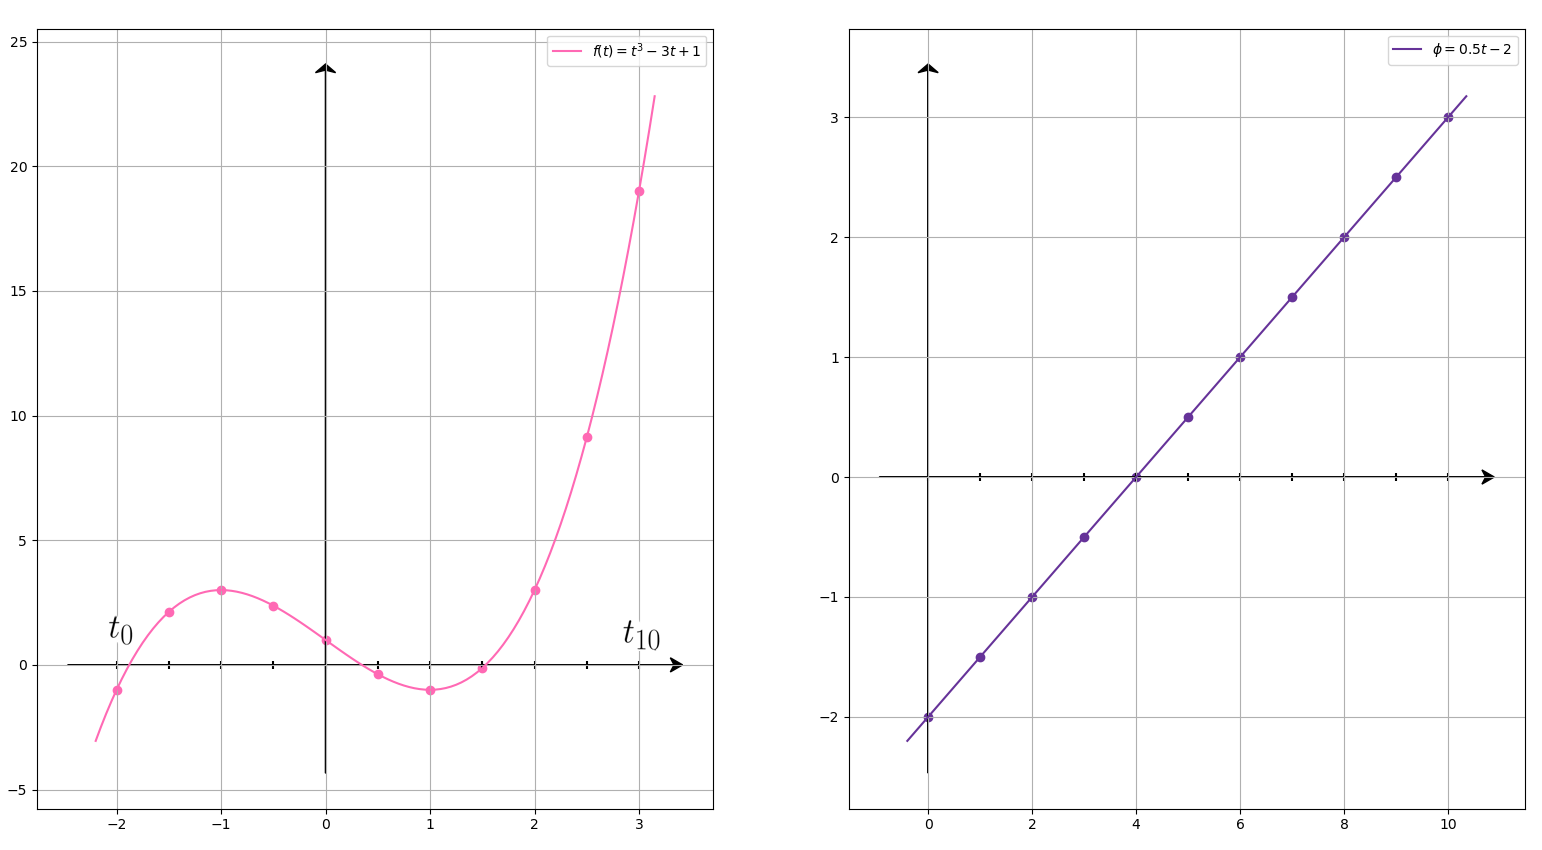
\includegraphics[scale=0.6]{mall} 
 \end{figure}
 
 
\begin{cor}
\label{cor: 18ap}
Sean $n\geq 2$, $0 \leq i \leq n-1$ enteros,
$\cali{P}$ una malla uniforme de $n$ puntos. 
Sea
\begin{equation*}
\label{def de espacios Wk}
W_{n,i}= span\{ v_{k} : 0 \leq k \leq i \},
\end{equation*}
el subespacio de $\IR^{n}$ 
definido en \eqref{espacios Wi}.
La señal
$x \in \IR^{n}$ es elemento de $W_{n,i}$ si y sólo si 
existe
$g(t) \in \IR[t]$ un polinomio de grado a lo más $i$
tal que 
$x = \Omega_{n, \cali{P}}(g)$.
\end{cor}
\noindent
\textbf{Demostración.}
En efecto, según la 
proposición \ref{obs: s en Wi sii es la discretizacion en malla Pn de un pol de grado a lo más i}, x es elemento de $W_{n,i}$ si y sólo si existe $q(t)$ polinomio
de grado a lo más $i$ tal que $x = \Omega_{n, \cali{P}_{n}}(q)$. Usando una función
de cambio de malla, se puede obtener a partir de $q$, componiendo con el 
cambio de malla, un polinomio $g(t)$ tal que 
$x = \Omega_{n, \cali{P}}(f)$.
\QEDB
\vspace{0.2cm}

\begin{prop} \label{Teorema1}
\textbf{(Caracterización de las bases
de los espacios $W_{n,i}$)} Sea $n \in \IN$.
Si $0 \leq i \leq n-1$ es un entero y
\[
\{ p_{k}=p_{k}(t): \hspace{0.2cm} 0 \leq k \leq i \}
\]
es una colección de polinomios con
\[
\partial (p_{k})=k, \hspace{0.4cm} 0 \leq k \leq i
\]
y 
\[
\cali{P}= \{ t_{j}= t_{0}+hj :\hspace{0.1cm} 0 \leq j \leq n-1 \}
\]
es una malla uniforme cualquiera
de $n$ puntos, entonces los $i+1$ vectores
de $\IR^{n}$
\begin{equation}
\label{eq1: 30Oct}
w_{k} := \Omega_{n, \cali{P}}(p_{k}), \hspace{0.4cm} 0 \leq k \leq i
\end{equation}
conforman una base del espacio $W_{n,i}$.

Recíprocamente, si $\cali{P}$ es una malla uniforme de $n$ puntos y
$\cali{B}_{i} := \{ w_{k} \}_{k=0}^{i}$
es una base de $W_{n,i}$, entonces 
\begin{itemize}
	\item[a)] todo $w_{k}$ es un polinomio discreto de dimensión $n$, 
	es decir, existe un polinomio $p_{k}$ de grado $k$ tal que 
	$w_{k} = \Omega_{n, \cali{P}}(p_{k})$,	
	y
	\item[b)] para cada $0 \leq k' \leq i$, uno y sólo uno de los polinomios
	$p_{k}$ tiene grado $k'$.
\end{itemize}
\end{prop}
\noindent
\textbf{Demostración.}
Según el corolario \ref{cor: 18ap}, 
$\{ w_{k}: \hspace{0.1cm} 0 \leq k \leq i \}$
es un subconjunto de $W_{n,i}$ de cardinalidad $i+1$; 
si demostramos que es 
linealmente independiente, puesto que por definición
$W_{n,i}$ es generado por $i+1$ vectores, podremos concluir,
como se quiere, que $\{ w_{k}: \hspace{0.1cm} 0 \leq k \leq i \}$
es base de $W_{n,i}$.
Sean $b_{k}$ con $0 \leq k \leq i$ escalares
para los que se tenga la siguiente igualdad en $\IR^{n}$:

\begin{equation} \label{eq1: 3Agosto}
\suma{k=0}{i}{b_{k}w_{k}}=0.
\end{equation}

\noindent 
Según la linealidad establecida en la observación
\ref{obs:linealidad de omega restringida a R[x]}
y la definición \eqref{eq1: 30Oct} de los vectores $w_{k}$,
si $p=p(t)$ es el polinomio
definido como
\begin{equation}
\label{eq2: 30Oct}
p:=\suma{k=0}{i}{b_{k}p_{k}},
\end{equation}
la ecuación \eqref{eq1: 3Agosto} puede reescribirse como

\begin{equation} \label{eq2: 3Agosto}
\Omega_{n , \cali{P}} (p) = 0;
\end{equation}

\noindent
por la proposición \ref{prop: consecuencia del TFA}
podemos inferir de esto que $p$ es el polinomio cero,  
o sea, que
$\suma{k=0}{i}{b_{k}p_{k}}$ es el polinomio cero,
y de esto, por la
independencia lineal de los polinomios $p_{i}$
en el espacio $\IR[t]$ (que se tiene por las condiciones
impuestas por hipótesis en los grados de estos), la
igualdad a cero de los escalares $b_{k}$. 

Recíprocamente, sea $\cali{B}_{i} := \{ w_{k} \}_{k=0}^{i}$
una base de $W_{n,i}$. Del corolario 
\ref{cor: 18ap} se sigue el punto a);
sean pues $p_{k}$, con $0 \leq k \leq i-1$, 
polinomios de grado
a lo más $i$ tales que 
$\Omega_{n, \cali{P}}(p_{k})=w_{k}$.
Supongamos que existe $0 \leq k' \leq i$
tal que ninguno de los polinomios $p_{k}$
tiene grado $k'$.

Sea $g_{k'}$ un polinomio cualquiera de grado $k'$.
Según el corolario \ref{cor: 18ap}, 
$z_{k'}:= \Omega_{n, \cali{P}}(g_{k^{'}})$ es elemento
de $W_{n,i}$; como $\cali{B}_{i} := \{ w_{k} \}_{k=0}^{i}$
es base de este espacio, existen escalares
$a_{k}$ (no todos cero, pues
$z_{k'} \neq 0$) tales que 
\[
z_{k'} = \suma{k=0}{i}{a_{k} w_{k}};
\]
evaluando el operador $\Omega_{n, \cali{P}}$ en ambos
lados de la igualdad y usando su linealidad
(c.f. observación \ref{obs:linealidad de omega restringida a R[x]}), 
obtenemos que 
\[
\Omega_{n, \cali{P}}
\left( g_{k'} - \suma{k=0}{i}{a_{k}p_{k}}
\right) = 0.
\]
Según la proposición
\ref{prop: consecuencia del TFA}, de esto se deduce que 
$g_{k'}$, un polinomio de grado $k'$, es 
igual a $\suma{k=0}{i}{a_{k}p_{k}}$, donde ninguno de los 
polinomios $p_{k}$ tiene grado $k'$.
Esto contradice la independencia lineal 
establecida en la observación 
\ref{obs:independencia lineal polinomios}.
\QEDB
\vspace{0.2cm}


\begin{cor}
Sea $n \in \IN$. Para todo entero $0 \leq i \leq n-1$, 
$\{v_{k}: \hspace{0.1cm} 0\leq k \leq i \}$ es una base
del espacio $W_{n,i}$
definido en \eqref{espacios Wi}.
\end{cor}


Las propiedades más importantes de los
espacios $W_{n,i}$ (y que se desprenden
de los argumentos anteriores) se 
resumen en el siguiente teorema. 
Sólo del notar que las dimensiones de 
$\IR^{n}$ y su subespacio $W_{n, n-1}$
coinciden se deduce el cuarto punto.


\begin{teo}
\label{cor: propiedades importantes de espacios Wi}
Sea $n \in \IN$. Sean, para cada $0 \leq i \leq n-1$,
los espacios $W_{n,i}$ como
se definieron en \eqref{espacios Wi}.
\begin{itemize}
\item Para toda $i$, $W_{n,i}$ es un subespacio
de $\IR^{n}$ de dimensión $i+1$. De hecho, 
$\{v_{k}: \hspace{0.1cm} 0\leq k \leq i \}$, con
$v_{k}$ definido como en \eqref{vectores vk},
es base de $W_{n,i}$.

\item La familia $(W_{n,i})_{i=0}^{n-1}$ de subespacios
	de $\IR^{n}$ está estrictamente anidada, es decir
	\begin{equation}
	\label{espacios Wi estan anidados}
	\forall \hspace{0.1cm}
	i = 0, \ldots , n-2: \hspace{0.2cm}
	W_{n,i} \subsetneq W_{n,i+1}.
	\end{equation}

\item 
Fijada una malla uniforme de $n$ puntos $\cali{P}$, 
para toda $x \in \IR^{n}$
se tiene que $x \in W_{n,i}$ si y sólo si
existe $g=g(x)$ un polinomio de grado a lo más $i$
tal que $x = \Omega_{n, \cali{P}}(g)$.

\item $\IR^{n}= W_{n,n-1}$.
\end{itemize}
\end{teo}

\begin{figure}[H]
\centering\captionsetup{format = hang}
	\begin{measuredfigure}
		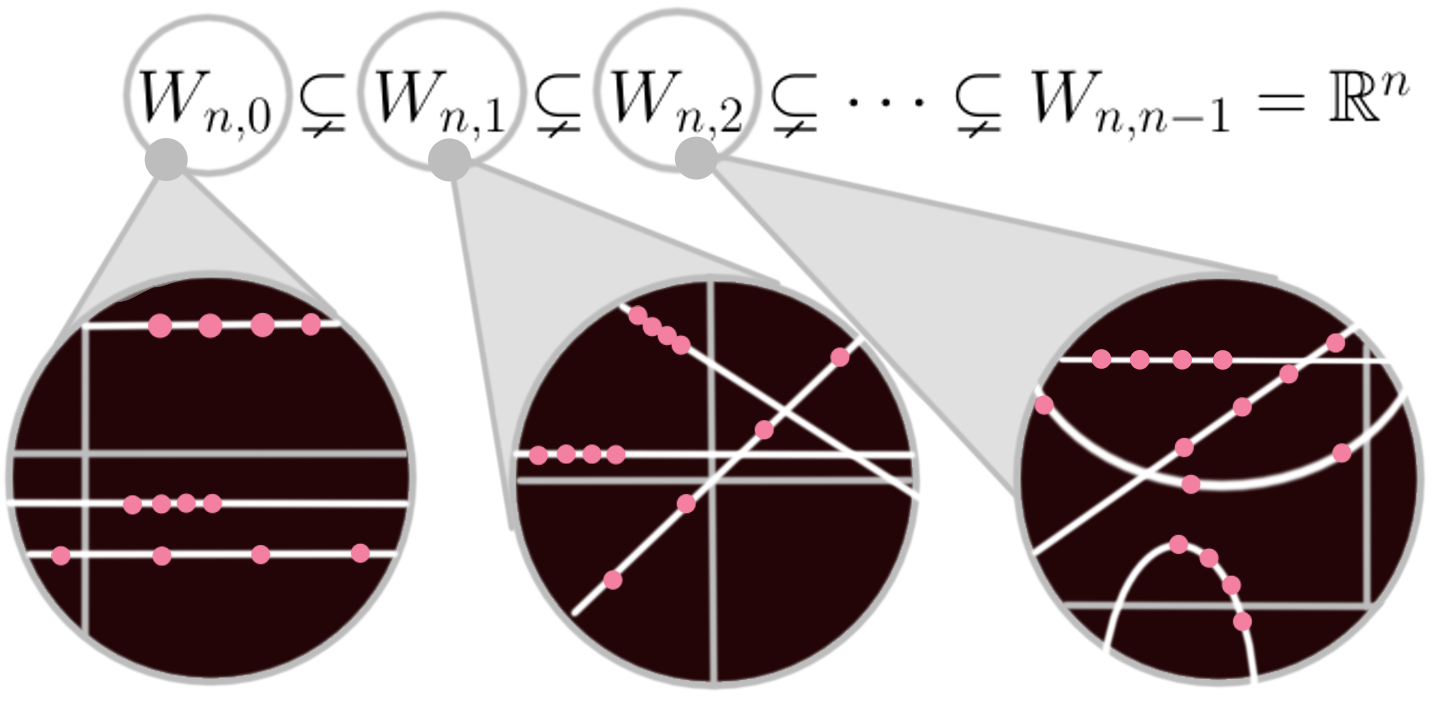
\includegraphics[scale=0.8]{nuevas_lupas} 
		\caption{
	En la figura	
	se dibujan las gráficas de algunos de los elementos
	de los tres primeros espacios de polinomios discretos
	$W_{n,0}$, $W_{n,1}$ y $W_{n,2}$
	(en la figura se ha fijado $n=4$).
    Observe que estas son
	las formas de recta y parábola de
	nuestro interés. 
	Queremos hacer énfasis en que, tomando
	\textbf{cualquier} malla uniforme y \textbf{cualquier} 
	polinomio $f$
	de grado $0 \leq i \leq n-1$, estamos seguros de que
	la discretización $\Omega_{n, \cali{P}}(f)$ es elemento
	del subespacio $W_{n,i}$ de $\IR^{n}$; reciprocamente, el 
	saber que un $x \in \IR^{n}$ sea elemento 
	de algún espacio $W_{n,i}$ (hecho
	que, en vistas de que la familia $(W_{n,i})_{i=0}^{n-1}$
	``cubre de manera ascendente a todo el espacio $\IR^{n}$''
	- c.f. puntos dos y cuatro del teorema 
	\ref{cor: propiedades importantes de espacios Wi}- seguro 
	ocurrirá), nos permite hacer inferencias sobre la forma 
	de la gráfica de $x$.}
 	\end{measuredfigure}
 \end{figure}





\section{Una definición del concepto de grado para señales finitas}
\label{definicion del concepto de grado para seniales finitas}

Revise nuevamente el último punto del teorema
\ref{cor: propiedades importantes de espacios Wi}; según este,
como se anticipó en la subsección 
\ref{discretizacion puntual, polinomios discretos y espacios asociados},
toda señal finita $x \in \IR^{n}$
es elemento de $W_{n,n-1}$,
es decir, es un polinomio discreto
de dimensión $n$ y grado menor a $n$.

Podemos dar una demostración
alternativa,
directa y sencilla de este hecho.

\begin{prop}
\label{prop: el operador de discretizacion puntual es un isomorfismo (...)}
Sean $n \in \IN$ y $\cali{P}$ 
una malla uniforme de $n$
puntos. 
La restricción del operador $\Omega_{n, \cali{P}}$
al espacio $\IR_{n-1}[t]$ de polinomios de grado a lo más
$n-1$, es decir, la función 
\begin{equation}
\label{eq0: 28Nov}
\Omega_{n, \cali{P}}:
\IR_{n-1}[t] \longrightarrow \IR^{n}
\end{equation}
es un isomorfismo de $\IR-$espacios vectoriales.
En particular, para todo vector $x \in \IR^{n}$
existe un único polinomio $f$ de grado menor a n
tal que $x = \Omega_{n, \cali{P}}(f)$.
\end{prop}
\noindent
\textbf{Demostración.}
Puesto que tanto $\IR_{n-1}[t]$
como $\IR^{n}$ son $\IR$-espacios vectoriales
de dimensión $n$, para ver que la función 
definida en
\eqref{eq0: 28Nov} (que, según la observación 
\ref{obs:linealidad de omega restringida a R[x]}, es lineal)
es un isomorfismo, basta
demostrar que es inyectiva 
(c.f. teorema 2.5 \cite{friedberg}).
Esto último es una consecuencia directa del 
teorema fundamental del álgebra,
pues, 
$f \in \IR_{n-1}[t]$
es elemento del kernel
de $\Omega_{n, \cali{P}}$ si y sólo si 
$\Omega_{n, \cali{P}}(f)=0$, o, equivalentemente,
si y sólo si 
cada uno de los $n$ puntos que componen la
malla $\cali{P}$ es una raíz de $f$;
según la proposición
\ref{prop: consecuencia del TFA},
esto último ocurre si y sólo si $f$ es el polinomio cero.
Con esto comprobamos que el kernel de la aplicación
\label{eq1: 25Nov} es trivial, luego, la inyectividad
de esta.
\QEDB
\vspace{0.2cm}

La proposición
\ref{prop: el operador de discretizacion puntual es un isomorfismo (...)}
parece sugerir 
una forma en la que podríamos 
definir el grado de 
un vector $x \in \IR^{n}$ (``dado $x \in \IR^{n}$, definimos
el grado de este como el grado del único polinomio $f \in \IR_{n-1}[t]$
tal que $\Omega_{n, \cali{P}}(f)=x$''); no hay
que apresurarse, pues en la formulación de
la proposición
\ref{prop: el operador de discretizacion puntual es un isomorfismo (...)}
se tuvo que fijar de antemano una malla uniforme.
\textit{A priori}, no podríamos descartar 
la existencia de mallas uniformes
$\cali{P}, \tilde{\cali{P}}$ 
de $n$ puntos
y de polinomios
$f, \tilde{f}$ de grados menores a $n$ (pero no 
iguales entre sí), tales que
$\Omega_{n, \cali{P}}(f) = x = \Omega_{n, \tilde{\cali{P}}}(\tilde{f})$.
Comprobamos que esto no ocurre
en la siguiente proposición.



\begin{ejemplo}
Lo que sí es seguro es que la unicidad establecida en la proposición \ref{prop: el operador de discretizacion puntual es un isomorfismo (...)} no es válida si se quita la restricción en los grados de los polinomios a discretizar.

Considere, por ejemplo a la señal
\[
x = (1,1,1) \in \IR^{3}.
\]
Los polinomios 
$f(t)=1$, $g(t)= 1-5t(t-0.4)(t-0.8)(t-1)(t-2)$
y $h(t) = 1+3t(t-1)(t-2)$,
de grados $0$, $5$ y $3$, respectivamente, son tales
que al ser evaluados en el operador
$\Omega_{3, \cali{P}_{3}}$ dan lugar a la señal $x$.

La señal 
\[
x = (1,1,0) \in \IR^{3}
\]
puede obtenerse como la discretización
del polinomio de grado $3$
$p(t) = 1+t(t-1)(t-2.5)$ en la  
malla uniforme $\cali{P}_{3}$, pero también como
la discretización del polinomio de grado $2$
$q(t)= 0.625 + t - 0.5t^{2}$
en la malla uniforme $\cali{P} = \{
0.5, 1.5, 2.5 \}$.

\begin{figure}[H]
	\sidecaption{
	Gráficas de los polinomios y señales de $\IR^{3}$
	expuestas en el ejemplo.
	\label{fig: restriccion en grado pol}
	}
	\centering
	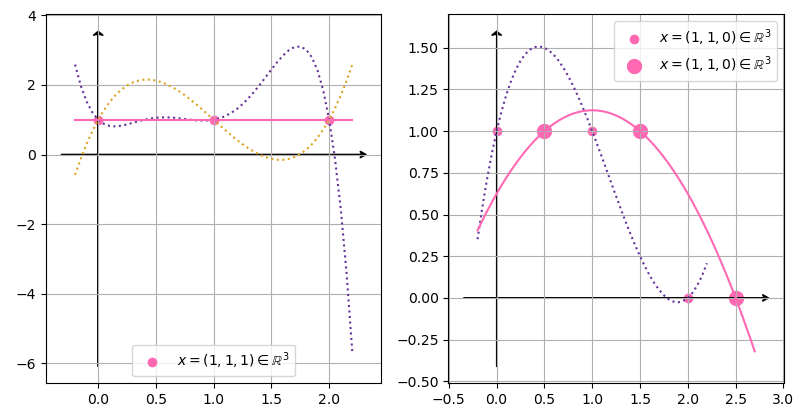
\includegraphics[scale=0.52]{25Nov_1} 
\end{figure}	
\final 
\end{ejemplo}


\begin{prop}
\label{prop: igualdad de grado (menor a n) si dos polinomios al discretizarse dan x}
Sean $n \in \IN$ y $x \in \IR^{n}$.
Si $\cali{P}, \tilde{\cali{P}}$ son mallas uniformes
de $n$ puntos y $\tilde{f}, f \in \IR_{n-1}[t]$
son tales que
\begin{equation}
\label{eq2: 25Nov}
\Omega_{n, \tilde{\cali{P}}}(\tilde{f})= x = 
\Omega_{n, \cali{P}}(f),
\end{equation}
entonces $\partial(\tilde{f})=\partial(f)$.
\end{prop}
\noindent
\textbf{Demostración.}
Digamos que 
\[
\cali{P}=\{t_{j}:=t_{0}+hj: \hspace{0.2cm} 0 \leq j \leq n-1 \},
\hspace{0.2cm}
\cali{\tilde{P}}=\{
\tilde{t}_{j}:=\tilde{t}_{0}+ \tilde{h}j: \hspace{0.2cm} 0 \leq j \leq n-1 \}.
\]
Sea 
\[
\phi(t)= \frac{h}{\tilde{h}}t+ \left( t_{0}-  \frac{h}{\tilde{h}}
\tilde{t}_{0}  \right)
\]
la función de cambio de malla
(de $\tilde{\cali{P}}$ a $\cali{P}$); esta función es 
tal que
\[
\forall \hspace{0.1cm} j = 0, \ldots, n-1, 
\hspace{0.5cm} \phi(\tilde{t}_{j})= 
t_{j};
\]
podemos reescribir entonces la hipótesis \eqref{eq2: 25Nov}
como 
\begin{align*}
(\tilde{f}(\tilde{t}_{0}), \ldots , \tilde{f}(\tilde{t}_{n-1}))
= & x \\
=& (f(t_{0}), \ldots , f(t_{n-1})) \\
=& ((f \circ \phi) (\tilde{t}_{0}), \ldots , 
(f \circ \phi) (\tilde{t}_{n-1})),
\end{align*}
o sea, como $\Omega_{n, \tilde{\cali{P}}}(\tilde{f})=
\Omega_{n, \tilde{\cali{P}}}(f \circ \phi)$; por linealidad
del operador $\Omega_{n, \tilde{\cali{P}}}$
(c.f. observación 
\ref{obs:linealidad de omega restringida a R[x]})
tenemos entonces que
$\Omega_{n, \tilde{\cali{P}}}(\tilde{f}-f \circ \phi)=0$.
Como 
$\tilde{f}-f \circ \phi$ es un polinomio de
grado menor a $n$, de esta
última igualdad podemos concluir, 
según la proposición
\ref{prop: consecuencia del TFA}, que
$\tilde{f}-f \circ \phi$
es el polinomio cero, por lo tanto
\begin{equation*}
\label{eq3: 25Nov}
\tilde{f}=f \circ \phi.
\end{equation*}

Puesto que el componer a $f$ con el polinomio lineal
$\phi$ no altera su grado (i.e. $f$ y $f \circ \phi$
son polinomios del mismo grado), concluimos que
\[
\partial(\tilde{f})= \partial(f \circ \phi)=
\partial(f).
\]
\QEDB
\vspace{0.2cm}

Con todo esto demostrado, podemos definir
el grado de una señal finita como sigue.


\marginnote{Nótese que el $f$ de la definición
\ref{def: del grado de una senial finita}
, según la proposición
\ref{prop: el operador de discretizacion puntual es un isomorfismo (...)},
siempre existe.}
\begin{defi}
\label{def: del grado de una senial finita}
Sean $n \in \IN$ y $x \in \IR^{n}$.
Si $f \in \IR_{n-1}[t]$
es un polinomio de grado menor a $n$
y $\cali{P}$ es una malla uniforme
de $n$ puntos tales que
$x= \Omega_{n, \cali{P}}(f)$, entonces
el \textbf{grado de $x$} es 
\[
\partial(x):= \partial(f).
\]
\end{defi}

Es fácil determinar el grado de una señal 
de dimensión $n$
en términos de pertencia a los espacios $W_{n,i}$;
mostramos a continuación que
el grado $i$ de un polinomio discreto es el índice
del menor subespacio $W_{n,i}$ en el que está contenido.

\begin{prop}
\label{prop: grado de x}
Sean $n \in \IN$ y $x \in \IR^{n}$ una señal de dimensión $n$.
\begin{itemize}
\item $x$ tiene grado cero si y sólo si $x \in W_{n,0}$.
\item Para toda $1 \leq i \leq n-1$,
$x$ tiene
grado $i$ si y sólo si 
$x \in W_{n,i}$ pero $x \not\in W_{n,i-1}$.
\end{itemize}
\end{prop}
\noindent
\textbf{Demostración.}
La veracidad del primer punto de la demostración
es obvia (pues $W_{n,0}$ consta exactamente de las discretizaciones
puntuales de polinomios constantes, c.f. 
teorema \ref{cor: propiedades importantes de espacios Wi}).
Demostremos pues el segundo punto.

\begin{itemize}
\item [$\Rightarrow$)]

Supongamos que $\partial(x)=i$ con $1 \leq i \leq n-1$;
por definición, esto significa que existen
$\cali{P}$ una malla uniforme de $n$ puntos y $f$ un 
polinomio 
tales que 
\begin{equation}
\label{eq5: 25Nov}
\partial(f)=i \hspace{0.2cm} \text{y} \hspace{0.2cm}
x=\Omega_{n,\cali{P}}(f).
\end{equation}
Según la proposición 
\ref{Obs1},
esto implica la pertenencia de $x$ a $W_{n,i}$.
Además, $x$ no puede ser elemento de $W_{n,i-1}$,
pues esto,
según el tercer punto del teorema
\ref{cor: propiedades importantes de espacios Wi},
implicaría la existencia de una
malla uniforme $\tilde{\cali{P}}$ de $n$
puntos y un polinomio $g$ tales que
\begin{equation}
\label{eq6: 25Nov}
\partial(g)\leq i-1 \hspace{0.2cm} \text{y} \hspace{0.2cm}
x=\Omega_{n,\tilde{\cali{P}}}(g);
\end{equation}
según la proposición
\ref{prop: igualdad de grado (menor a n) si dos polinomios al discretizarse dan x}, \eqref{eq5: 25Nov}
y \eqref{eq6: 25Nov} no pueden ser ambas verdaderas.

\item[$\Leftarrow$)] Sea
$1 \leq i \leq n-1$ tal que $x \in W_{n,i}$
pero $x \not\in W_{n,i-1}$.
Según el teorema
\ref{cor: propiedades importantes de espacios Wi}, existen
$\cali{P}$ malla uniforme de $n$ puntos y
$f$ polinomio de grado a lo más $i$ tales que
$x= \Omega_{n, \cali{P}}(f)$; según este mismo
teorema, el que el grado de $f$ fuese menor a $i$
implicaría que $x$ también fuese elemento
del espacio $W_{n,i-1}$. Como esto no ocurre, concluimos
que $x= \Omega_{n, \cali{P}}(f)$
con $\partial(f)=i$, luego, según la definición
\ref{def: del grado de una senial finita}, 
$x$ tiene grado $i$. \QEDB
\end{itemize}
\vspace{0.2cm}

Terminamos con una definición, que queda justificada
por lo establecido en la proposición \ref{prop: grado de x}.

\begin{defi}
Sean $n \geq 2$, $0 \leq i \leq n-1$ enteros. 
Al subespacio $W_{n,i}$ definido en \eqref{espacios Wi}
se le denominará el \textbf{espacio de señales $n-$dimensionales
de grado a lo más $i$.}
\end{defi}



\section{Construcción canónica de las bases de Legendre discretas}

\noindent Ahora, con el 
algoritmo de Gram-Schmidt (descrito
en la proposición \ref{Prop:Gram-Schmidt2})
vamos a normalizar
a la base $\{v_{k}: \hspace{0.1cm} 0 \leq k \leq n-1 \}$ de
$W_{n,n-1}$, o sea, de $\IR^{n}$ (c.f. 
cuarto punto del teorema
\ref{cor: propiedades importantes de espacios Wi}). 
Por la naturaleza del proceso, durante este se
obtienen bases ortonormales para cada uno de los espacios 
$W_{n,i}$, pues los espacios $W_{n,i}$ están anidados y dos consecutivos
de estos difieren por uno en dimensión; en este contexto, realizar
el $k-$ésimo paso en el algoritmo de ortonormalización de Gram-Schmidt
lleva a calcular una base ortonormal para el $k-$ésimo espacio $W_{n,i}$.

%\begin{figure}[H]
%   \centering
%   \incfig{28JunioInks}
%    \caption{ 
%    \TODO{Cambiar notación espacios W}
%    Como muestra el diagrama, 
%	lo que se hace es proyectar el vector $v_{k}$, con
%	$1 \leq k \leq n-1$, al espacio
%	$W_{n,k-1}$ para así 
%	formar al vector $\bar{\xi}_{k}$ y después
%	normalizarlo.}
%\end{figure}



\begin{defi} 
\label{def: base de Legendre discreta}
A la base ortonormal de $\IR^{n}$
\begin{equation}
\label{eq: base de Legendre discreta}
\cali{L}^{n}=\{ \cali{L}^{n,k}= (\cali{L}_{m}^{n,k})_{m=0}^{n-1} \in \IR^{n}: 
\hspace{0.1cm} 0 \leq k \leq n-1\}
\end{equation}
que resulta de ortonormalizar con G-S a la base
\[
\{v_{k} \in \IR^{n}: \hspace{0.1cm} 0 \leq k \leq n-1 \}
\]
de $\IR^{n}$ la llamaremos la
\textbf{base de Legendre discreta de dimensión $n$}.

Denominaremos a la señal $\cali{L}^{n,k}$ el 
\textbf{polinomio discreto de Legendre de dimensión
$n$ y grado $k$}.
\end{defi}

\begin{nota}
A partir de ahora, abreviaremos el nombre
``polinomio discreto de Legendre''
como ``PDL'' y ``base de Legendre discreta'' como ``BLD''.
\end{nota}

\begin{cor} \label{cor: BON de legendre para espacios Wk}
Sea $n \in \IN$. Para todo $0 \leq k \leq n-1$, los vectores
\[
\cali{L}^{n, l}, \hspace{0.2cm} 0 \leq l \leq k
\]
conforman una BON del espacio $W_{n,k}$.
\end{cor}

\begin{cor} \label{cor: Ln,k ortogonal a todo pol discreto de grado menor a k}
Sea $n \in \IN$. Si $k$ es un entero con $1 \leq k \leq n-1$,
entonces
\[
\forall \hspace{0.1cm} 0 \leq l \leq k-1:
\hspace{0.2cm}
\cali{L}^{n,k} \in W_{n,l}^{\perp},
\]
o sea, 
$\cali{L}^{n,k}$ es ortogonal a todo polinomio discreto
de grado menor a $k$.
\end{cor}
\noindent
\textbf{Demostración.}
En efecto, según la definición
\ref{def: base de Legendre discreta}, 
$\cali{L}^{n,k}$ es ortogonal a todos los vectores
$\cali{L}^{n, l}$ con $0 \leq l \leq k-1$,
luego, según el corolario
\ref{cor: BON de legendre para espacios Wk},
es
ortogonal a todos los elementos
de una base del espacio $W_{n,l}$,
por lo tanto, a todo elemento de este.
\QEDB
\vspace{0.2cm}



\begin{figure}[H]
	\sidecaption{
	Dado el polinomio discreto de Legendre $\cali{L}^{n,k}=(\cali{L}^{n,k}_{m})$,
	$n$ es la variable de \textbf{dimensión}, 
	$k \in \{0,\ldots,n-1 \}$ la de 
	\textbf{grado} y $m$ es el índice de \textbf{posición.}
	\label{fig: pdl}
	}
	\centering
	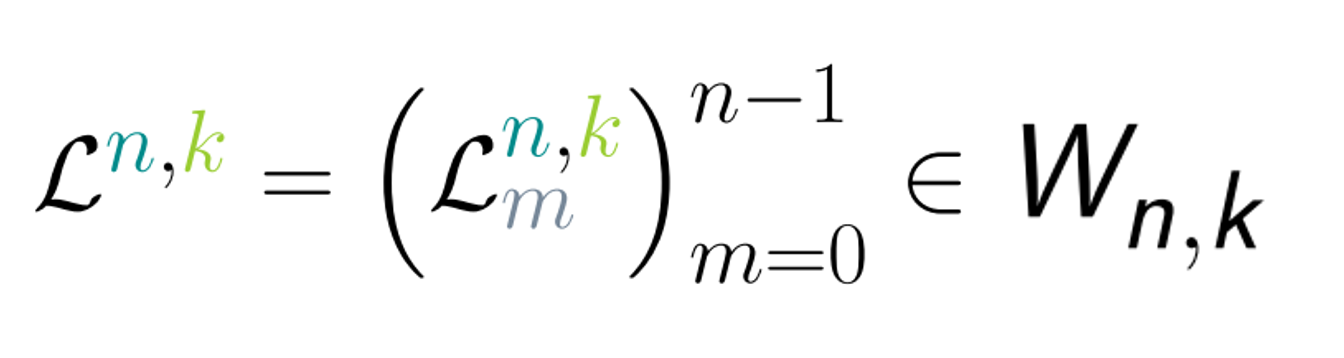
\includegraphics[scale= 0.35]{pdl} 
\end{figure}	


\begin{nota}
Observe la analogía entre nuestra construcción de la BLD
con la esbozada en el capítulo 
\ref{chapter: introduccion} sobre la construcción 
usual de los polinomios
de Legendre (de variable continua);
en ambos casos partimos de familias anidadas de espacios 
de polinomios
(discretos o continuos, dependiendo del caso);
	\[
	\{ W_{n,k} \}_{k=0}^{n-1} 
	\]
para el caso discreto, y
	\[
	\{ \IR_{k,-1,1} \}_{k \in \overline{\IN}}
	\]	
para el caso continuo (c.f. \ref{notacion: 17ap}),
y, con el 
método de Gram-Schmidt, ortonormalizamos estas bases para obtener
una BON del espacio ambiente que contiene a la familia
(que es $\IR^{n}$ en el primer caso y $L^{2}[-1,1]$
en el segundo). \\

Observe sin embargo que, en el caso discreto, además
del parámetro de grado $k$ se tiene también un parámetro
$n$ de dimensión. Otra diferencia es que, en el caso 
continuo, se trataba con una familia anidada numerable, mientras
que en el caso $n-$dimensional la familia anidada consta
de $n$ miembros.
\end{nota}


\begin{comment}
{\Huge{
$\cali{L}^{\textcolor{ameCyanO}{n}, \textcolor{ameVerde}{k}} =
\left(
\cali{L}^{\textcolor{ameCyanO}{n}, \textcolor{ameVerde}{k}}_{
\textcolor{ameGris}{m}}
\right)_{m=0}^{n-1} \in \IR^{n }
$
}}
\end{comment}

\begin{ejemplo}
A continuación, mostramos las gráficas de los
elementos de las bases $\cali{L}^{2}$ y $\cali{L}^{3}$.

\begin{figure}[H]
	\sidecaption{
	Gráficas de los elementos de $\cali{L}^{2}
	\subseteq \IR^{2}$.
	\label{fig: graficas elementos L2}
	}
	\centering
	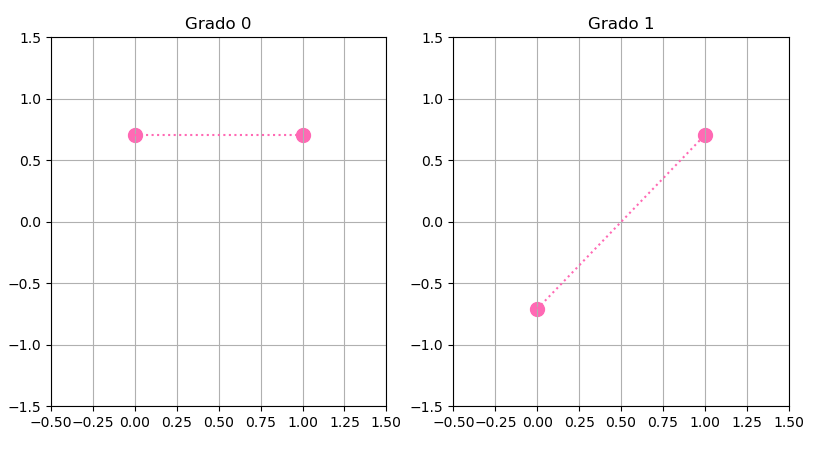
\includegraphics[scale=0.5]{graficasLegendre2} 
\end{figure}	


\begin{figure}[H]
	\sidecaption{
	Gráficas de los elementos de $\cali{L}^{3} 
	\subseteq \IR^{3}$.
	\label{fig: graficas elementos L2}
	}
	\centering
	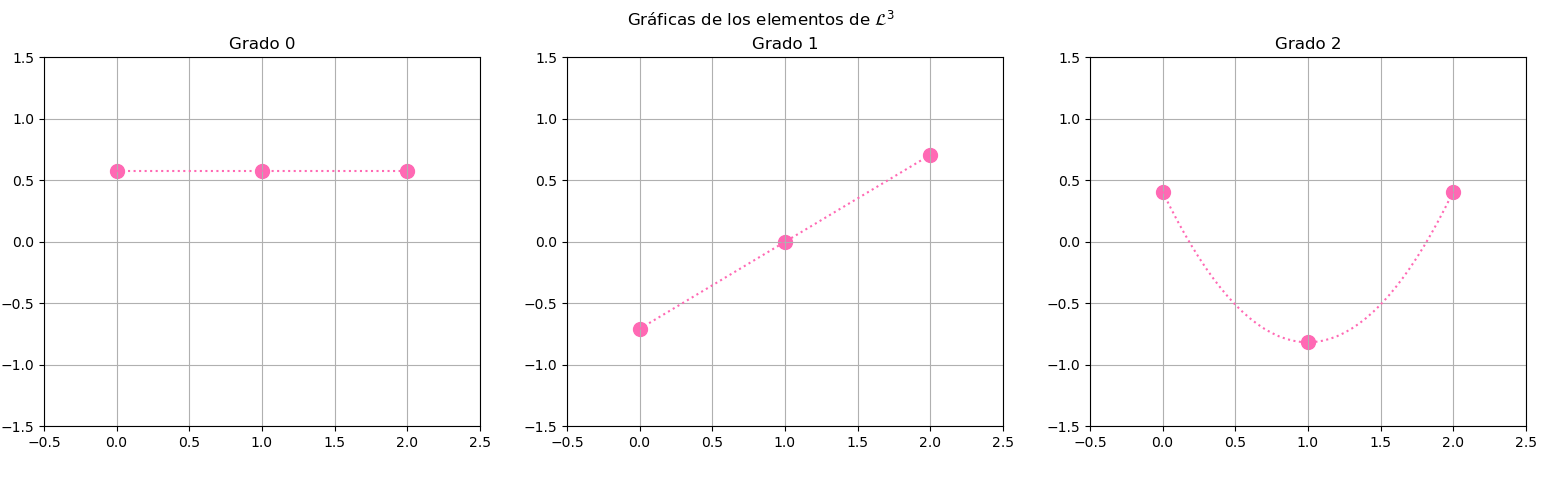
\includegraphics[scale=0.3]{graficasLegendre3} 
\end{figure}	 




En el caso $n=2$, el único subespacio de polinomios
discretos no trivial es 
\begin{align*}
W_{2,0}= & span \left\{ 
\left(\frac{1}{\sqrt2}, \frac{1}{\sqrt2} \right) \right\} \\
= & \{ (x,x) \in \IR^{2}: \hspace{0.2cm} x \in \IR \},
\end{align*}

pues

\begin{equation*}
\label{eq1: 1Dic}
W_{2,1}= \IR^{2}.
\end{equation*}


En el caso $n=3$, calculamos que
\begin{align*}
W_{3,0}= & span \left\{
\left( \frac{1}{\sqrt3}, \frac{1}{\sqrt3},
\frac{1}{\sqrt3} \right) \right\}  \\
= & \{ (x,x,x) \in \IR^{3}: \hspace{0.2cm} x \in \IR \},
\end{align*}

\begin{align}
\label{eq2: 1Dic}
W_{3,1}= & span \left\{ \left( \frac{1}{\sqrt3}, \frac{1}{\sqrt3},
\frac{1}{\sqrt3} \right) ,
\left( -\frac{1}{\sqrt2}, 0,  \frac{1}{\sqrt2} \right) \right\}
\nonumber \\
= & \{ (x,y,2y-x) \in \IR^{3}: \hspace{0.2cm} x,y \in \IR \},
\end{align}
y
\[
W_{3,2}=\IR^{3}.
\]

\begin{figure}[H]
	\sidecaption{
	Gráficas de 
	$W_{2,0} \subseteq \IR^{2}$
	y de los subespacios
	$W_{3,0}$ y $W_{3,1}$ de $\IR^{3}$ que
	son, respectivamente, una recta y un plano;
	observe que
	$W_{3,0} \subseteq W_{3,1}$ y que tanto 
	$W_{2,0}$ como $W_{3,1}$ dividen en dos regiones
	ajenas a sus correspondientes espacios ambiente.
	\label{fig: graficas espacios W para dimensiones 2 y 3}
	}
	\centering
	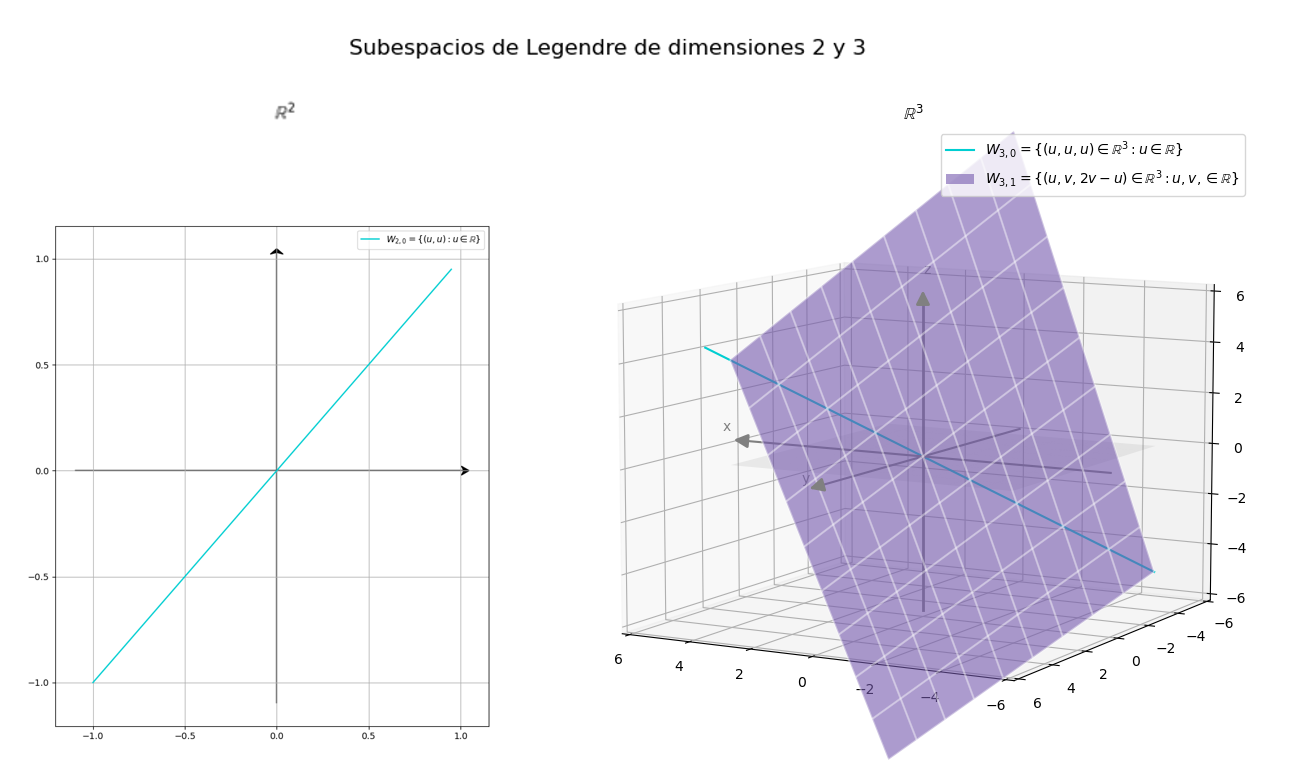
\includegraphics[scale= 0.38]{legendre2y3} 
\end{figure}	

\final
%final ejemplo 1--------------------------------------------
\end{ejemplo}



\section{Sobre formas alternativas de definición de la base $\cali{L}^{n}$}

Ahora,
fijada una dimensión $n$,
vamos a generalizar los tipos de objetos
usados
en el método por medio del cual
se definió a la base de Legendre discreta $\cali{L}^{n}$
(en la subsección 
\ref{Generalización que involucra a la discretización Omega n}),
y además, como prometimos en la introducción,
vamos a dar una segunda forma natural de
de abordar el problema, cambiando el método de 
discretización
(en la subsección 
\ref{Construcción de Ln en base a discretizaciones con sumas integrales}),
llegando, como se anticipó, a la base
$\cali{L}^{n}$.

\subsection{Generalización que involucra a la discretización $\Omega_{n}$}
\label{Generalización que involucra a la discretización Omega n}

Recuerde que, al definir a los espacios
de polinomios discretos
$W_{n,i}$ en \eqref{def de espacios Wk},
consideramos a
las funciones polinomiales 
$f_{k}(t)=t^{k}$, con $0 \leq k \leq n-1$, que después
discretizamos en la malla uniforme
$\cali{P}_{n}= \{ j: \hspace{0.1cm} 0 \leq j \leq n-1 \} $
para obtener los vectores $v_{k}$; nos
disponemos a probar que, si hubiésemos escogido
\begin{itemize}
\item funciones polinomiales
\[
g_{k}(t) \in \IR[x], \hspace{1cm} 
\text{con }\hspace{0.5cm} 0 \leq k \leq n-1 \hspace{0.2cm} \text{entero},
\]
donde
el grado de $g_{k}$ es $k$ y su coeficiente principal 
$c_{k}$ es positivo, y

\item cualquier malla uniforme de $n$ puntos
\[
\cali{P}=\{t_{j} : \hspace{0.1cm} 0 \leq j \leq n-1 \},
\]
\end{itemize}
si 
\begin{equation}
\label{eq1: 31Oct}
w_{k} := \Omega_{n,\cali{P}}(g_{k})
=(g_{k}(t_{j}))_{j=0}^{n-1}, \hspace{0.3cm} 0 \leq k \leq n-1,
\end{equation}
entonces estos vectores $w_{k}$
generan a los mismos espacios $W_{n,i}$
de antes y,
después de ortonormalizar con el 
método de Gram-Schmidt
al subconjunto $\{w_{k}: \hspace{0.2cm} 0 \leq k \leq n-1\}$
de $\IR^{n}$, obtendríamos la 
base de Legendre discreta $\cali{L}^{n}$ 
definida en \eqref{eq: base de Legendre discreta}. 



\begin{ej}
Sea $n=3$; sean las colecciones de polinomios
\begin{equation}
\label{eq11: 10Dic}
\{
f_{0}(t), 
f_{1}(t), f_{2}(t) \},
\end{equation}
con los polinomios $f_{k}$ como se definieron en \eqref{fk}, y
\begin{equation}
\label{eq12: 10Dic}
\left\{
g_{0}(t):=3,  
g_{1}(t):=\frac{1}{2}t+1,
g_{2}(t):=t^{2}+2t+3 \right\}.
\end{equation}



\begin{figure}[H]
\centering\captionsetup{format = hang}
	\begin{measuredfigure}
		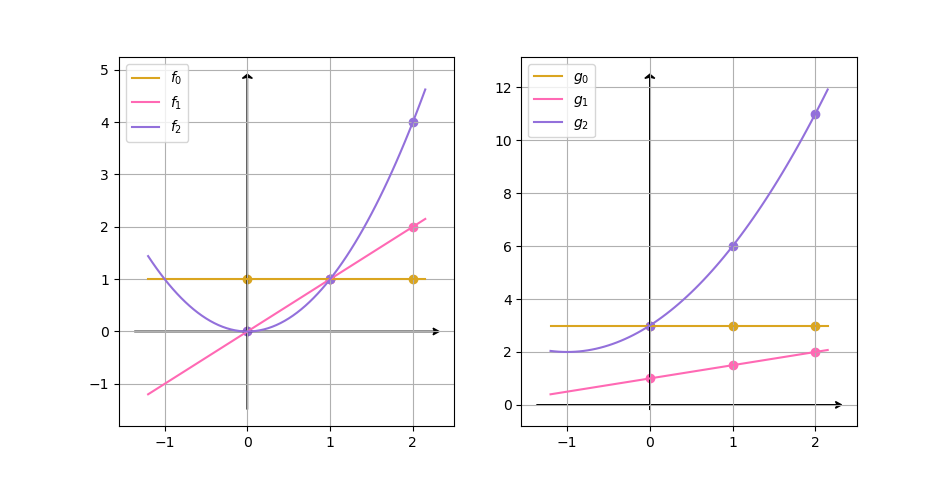
\includegraphics[scale=0.6]{EsquemaGral} 
		\caption{Ejemplo concreto del proceso tomando 
		las dos colecciones
    de polinomios \eqref{eq11: 10Dic} y \eqref{eq12: 10Dic},
    (que tienen en común que contienen, por cada $0 \leq k \leq 2$,
    un polinomio de grado $k$ y coeficiente principal positivo), y
    discretizándolas, respectivamente, en las mallas uniformes 
    $\cali{P}_{3}$ y $\cali{P} =\{-2, -\frac{1}{2}, 1 \}$.}
 	\end{measuredfigure}
 \end{figure}


Afirmamos que, si
\begin{itemize}
\item \textcolor{ameMorado}{{(Discretización)}}
consideramos, para $0 \leq k \leq 2$, a los vectores
\[
v_{k}:= \Om_{3, \cali{P}_{3}}(f_{k})
\hspace{0.2cm} \text{y} \hspace{0.2cm}
w_{k}:= \Om_{3, \cali{P}}(g_{k}),
\]
\item \textcolor{ameMorado}{{(Ortogonalización)}}
en base a estos definimos a los vectores
$$ \bar{\xi}_{0}:= v_{0}, 
\hspace{0.2cm} \bar{\eta}_{0}:= w_{0}, 
$$
$$ \bar{\xi}_{k}:= v_{k} - \Pi_{W_{k-1}}(v_{k}), \hspace{0.2cm}
\bar{\eta}_{k}:= w_{k} - \Pi_{W_{k-1}}(w_{k})
\hspace{0.2cm} \text{para} 
\hspace{0.1cm}
k=1,2, $$ y, finalmente, 
\item \textcolor{ameMorado}{{(Normalización)}}
definimos, para toda $0 \leq k \leq 2$,
a los vectores
$$\xi_{k}:= \frac{\bar{\xi}_{k}}{|| \bar{\xi}_{k} ||},
\hspace{0.2cm}
\eta_{k}:= \frac{\bar{\eta}_{k}}{|| \bar{\eta}_{k} ||},
$$
\end{itemize}
entonces, ocurre que
\[
\forall \hspace{0.1cm} 0 \leq k \leq 2:
\hspace{0.2cm} \xi_{k}= \eta_{k}.
\]
\final
\end{ej}



%\begin{tcolorbox}[title=Ejemplo]

%	\begin{figure}[H]
%	\centering
%	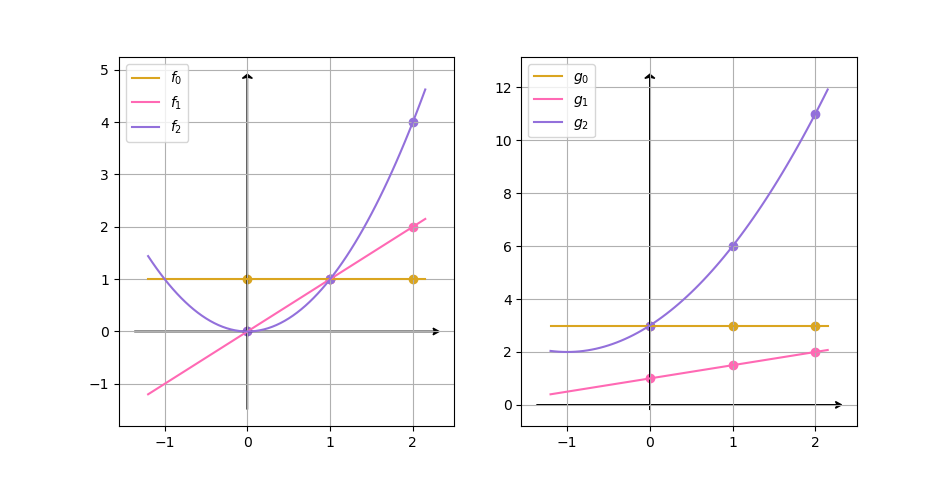
\includegraphics[scale=0.45]{EsquemaGral}
%	\caption{Ejemplo concreto del proceso tomando dos colecciones
 %   de polinomios (a saber, $f_{0}$,  $f_{1}$, $f_{2}$,
  %  y $g_{0}(t):=3$, $g_{1}(t):=\frac{1}{2}t+1$, $g_{2}(t):=t^{2}+2t+3$)
 %   discretizándolas, respectivamente, en las mallas uniformes 
 %   $\cali{P}_{3}$ y $\cali{P} =\{-2, -\frac{1}{2}, 1 \}$.}
%	\end{figure}	

%\tcblower
%\begin{center}
%1.- Discretización
%\end{center}
%\begin{tcbitemize}[raster equal height,colframe=white,colback=white,
%raster every box/.style={minimum for current equal height group=2cm}]
%\tcbitem Consideramos a los vectores
%$$v_{k}:= \Om_{3, \cali{P}_{3}}(f_{k}),$$ con
%$k=0,1,2$.
%\tcbitem Consideramos a los vectores
%$$w_{k}:= \Om_{3, \cali{P}}(g_{k}),$$ con
%$k=0,1,2$.
%\end{tcbitemize}

%\DrawLine

%\begin{center}
%2.- Gram-Schmidt
%\end{center}
%\begin{tcbitemize}[raster equal height,colframe=white,colback=white,
%raster every box/.style={minimum for current equal height group=2cm}]
%\tcbitem Definimos a los vectores
%$$ \bar{\xi}_{0}:= v_{0}, $$
%$$ \bar{\xi}_{k}:= v_{k} - \Pi_{W_{k-1}}(v_{k}),
%\hspace{0.2cm} k=1,2. $$

%\tcbitem Definimos a los vectores
%$$ \bar{\eta}_{0}:= w_{0}, $$
%$$ \bar{\eta}_{k}:= w_{k} - \Pi_{W_{k-1}}(w_{k}),
%\hspace{0.2cm} k=1,2. $$
%\end{tcbitemize}


%\DrawLine

%\begin{center}
%3.- Normalización
%\end{center}
%\begin{tcbitemize}[raster equal height,colframe=white,colback=white,
%raster every box/.style={minimum for current equal height group=2cm}]
%\tcbitem Definimos a los vectores
%$$ \xi_{k}:= \frac{\bar{\xi}_{k}}{|| \bar{\xi}_{k} ||},
%\hspace{0.2cm} k=0,1,2. $$

%\tcbitem Definimos a los vectores
%$$ \eta_{k}:= \frac{\bar{\eta}_{k}}{|| \bar{\eta}_{k} ||},
%\hspace{0.2cm} k=0,1,2. $$
%\end{tcbitemize}
%\DrawLine
%\begin{center}
%Afirmación
%\end{center}
%\begin{tcolorbox}[use height from group=C,add to height=-2cm,
%colframe=white,colback=white]
%\begin{center}
%$\forall \hspace{0.1cm} 0 \leq k \leq 2: \hspace{0.2cm} \xi_{k}=\eta_{k}$.
%\end{center}
%\end{tcolorbox}
%\end{tcolorbox}







\begin{itemize}
\item[\textbf{Paso I}] 
Primero demostremos que vectores $w_{k}$ así
construidos forman bases para los espacios
de polinomios discretos.
\begin{prop}
\label{prop: los wk forman bases de los Wnk}
Sea 
\begin{equation}
\label{eq5: 2En}
\{g_{k}: \hspace{0.2cm} 0 \leq k \leq n-1 \} 
\end{equation}
una colección
de polinomios, con $g_{k}$ un polinomio de grado $k$ y coeficiente 
principal positivo. Sean 
$\cali{P}$ una malla uniforme de $n$ puntos y 
considere a los vectores $w_{k}$ 
definidos en \eqref{eq1: 31Oct}.
Para toda $0 \leq i \leq n-1$, los vectores
\[
w_{k} \hspace{0.2cm} \text{con } 0 \leq k \leq i
\]
conforman una base del espacio $W_{n,i}$.
\end{prop}
\noindent
\textbf{Demostración.}
Observe que el subconjunto \eqref{eq5: 2En}
de $\IR[x]$
es linealmente independiente 
en tal espacio (por cuestión de grados,
ningún $g_{k}$ puede expresarse como combinación lineal de
los anteriores); así, según 
la proposición \ref{Teorema1},
para toda $0 \leq k \leq n-1$, los $n$ vectores $w_{k}$
de $\IR^{n}$ 
definidos en 
\eqref{eq1: 31Oct}
son linealmente independientes en $\IR^{n}$.

Puesto que
los $i+1$ primeros de ellos son elementos del 
espacio $W_{n,i}$
(c.f. proposición \ref{Obs1}) y 
como $dim(W_{n,i})=i+1$
(c.f. teorema \ref{cor: propiedades importantes de espacios Wi}), 
estos $i+1$ vectores conforman
una base del espacio $W_{n,i}$.
\QEDB
\vspace{0.2cm}


\item[\textbf{Paso II}] 
Tenemos entonces dos bases de 
$W_{n,n-1}=\IR^{n}$:
\begin{equation}
\label{eq2: 31Oct}
\{v_{i} : \hspace{0.1cm} 0 \leq i \leq n-1 \} \subseteq \IR^{n}
\hspace{0.25cm} \text{y} \hspace{0.25cm}
\{w_{i} : \hspace{0.1cm}  0 \leq i \leq n-1 \}\subseteq \IR^{n},
\end{equation}

donde, recuerde, los vectores $v_{i}$ se definen como en
\ref{notacion: Pn, fk, Wi, vk}
y los $w_{i}$ son las discretizaciones definidas en
\eqref{eq1: 31Oct}.
Sean
\begin{equation}
\label{eq3: 31Oct}
\{\bar{\xi_{i}}: \hspace{0.1cm}  0 \leq i \leq n-1 \}
\hspace{0.25cm} \text{y} \hspace{0.25cm}
\{\bar{\eta_{i}}: \hspace{0.1cm}  0 \leq i \leq n-1 \}
\end{equation}

las bases que resultan de ortogonalizar a 
las bases dadas en \eqref{eq2: 31Oct} con G-S, y 
\begin{equation}
\label{eq4: 31Oct}
\{\xi_{i}: \hspace{0.1cm} 0 \leq i \leq n-1  \}, \hspace{0.5cm}
\{\eta_{i}: \hspace{0.1cm} 0 \leq i \leq n-1 \}
\end{equation}
a las normalizaciones de las bases dadas en 
\eqref{eq3: 31Oct}, o sea, a las bases cuyos elementos son,
respectivamente,
\begin{equation}
\label{eq0: 1En}
\xi_{i}:= \frac{\overline{\xi_{i}}}{||\overline{\xi_{i}}||}
\hspace{0.5cm} \text{y} \hspace{0.5cm}
\eta_{i}:= \frac{\overline{\eta_{i}}}{||\overline{\eta_{i}}||}
\end{equation}
con $0 \leq i \leq n-1$.

De la definición de los vectores \eqref{eq0: 1En}
y el teorema \eqref{cor: propiedades importantes de espacios Wi} se
sigue inmediantamente lo siguiente:

\begin{obs}
\label{obs: los xi y los etai son elementos de Wni}
Sea $n \in \IN$. Para cada $0 \leq i \leq n-1$, los vectores
$\xi_{i}$ y $\eta_{i}$ 
definidos en \eqref{eq0: 1En} son elementos del
subespacio $W_{n, i}$ de $\IR^{n}$.
\end{obs}

La importancia del \textbf{Paso I} es que, 
para efectuar los dos
procesos de G-S necesarios para
construir las bases 
\eqref{eq3: 31Oct}, a pesar de que trabajaremos
con dos bases distintas de $\IR^{n}$,
vamos a estar proyectando siempre sobre 
los mismos espacios $W_{n,i}$.
Esta observación es clave para la 
demostración de la siguiente proposición.


\begin{prop} \label{prop:signo}
Sea $n \in \IN$.
Para $0 \leq i \leq n-1$, sean los vectores $\xi_{i}$
y $\eta_{i}$ como en \eqref{eq4: 31Oct}.
Para toda $i$, $\xi_{i}= \pm \eta_{i}$.
\end{prop}
\noindent
\textbf{Demostración.}
La clave de la demostración
radicará en ``atrapar'' en un mismo espacio de 
dimensión uno a los vectores
unitarios $\xi_{i}$ y $\eta_{i}$ de $\IR^{n}$. 


Sea $i=0$. Según el teorema de Gram-Schmidt
\ref{Prop:Gram-Schmidt2}, $\overline{\xi_{0}}=v_{0}$
y $\overline{\eta_{0}}=w_{0}$; además,
por definición, $v_{0}$ es
el vector constante uno, y
$w_{0}$ es la discretización (en una malla uniforme $\cali{P}$)
de un polinomio constante $g(t)=c_{0}$ con $c_{0}>0$.
Usando esto y la definición \eqref{eq0: 1En}
tenemos que

\[
\xi_{0}=
\frac{\overline{\xi_{0}}}{||\overline{\xi_{0}}||}=
\frac{v_{0}}{||v_{0}||}=\frac{(1, \ldots , 1)}{\sqrt{n}}=
\frac{(c_{0}, \ldots , c_{0})}{c_{0}\sqrt{n}}= \frac{w_{0}}{||w_{0}||}=
\frac{\overline{\eta_{0}}}{||\overline{\eta_{0}}||}=\eta_{0},
\]
o sea, la veracidad de la proposición para $i=0$.



Sea ahora $1 \leq i \leq n-1$.
Según la definición de los espacios
$W_{n,i}$ dada en \eqref{espacios Wi}
y lo notado en el \textbf{Paso I},
\[
span\{ v_{k}: \hspace{0.1cm} 0 \leq k \leq i \}=W_{n,i}=
span\{ w_{k}: \hspace{0.1cm} 0 \leq k \leq i \},
\]
luego, según la definición de las bases
\eqref{eq4: 31Oct}
el teorema de Gram-Schmidt
\ref{Teo:Gram-Schmidt},

\[
span\{ \xi_{k}: \hspace{0.1cm} 0 \leq k \leq i \}=
W_{n,i} =span\{ \eta_{k}: \hspace{0.1cm} 0 \leq k \leq i \}.
\]
\noindent
Similarmente,
\[
span\{ \xi_{k}: \hspace{0.1cm} 0 \leq k \leq i-1 \}=
W_{n,i-1} =span\{ \eta_{k}: \hspace{0.1cm} 0 \leq k \leq i-1 \}.
\]

Recuerde ahora que el espacio $W_{n,i-1}$
está contenido en $W_{n,i}$
(c.f. teorema \ref{cor: propiedades importantes de espacios Wi});
si por $V_{n,i}$ denotamos al complemento ortogonal de $W_{n,i-1}$
no respecto a $\IR^{n}$, sino 
respecto a $W_{n,i}$, i.e. si
\begin{equation}
\label{eq1: 1En}
V_{n,i} := W_{n,i} \ominus W_{n,i-1},
\end{equation}
entonces, como 
$dim(W_{n,i})=i+1$ y $dim(W_{n,i-1})=i$
(c.f. teorema \ref{cor: propiedades importantes de espacios Wi}), 
$V_{n,i}$ es un espacio
vectorial de dimensión uno
(c.f. \TODO{apéndice,}). Ahora bien,

\begin{itemize}
\item como se notó en la observación 
\ref{obs: los xi y los etai son elementos de Wni},
$\xi_{i}$ es un elemento de $W_{n,i}$ que,
según el teorema de Gram-Schmidt \ref{Teo:Gram-Schmidt},
es ortogonal
a $\xi_{0}, \ldots , \xi_{i-1}$, luego, 
según la ecuación \eqref{eq1: 1En},
$\xi_{i} \in V_{n,i}$.

\item Dualmente, $\eta_{i} \in V_{n,i}$.
\end{itemize}

En conclusión, $\xi_{i}$ y $\eta_{i}$ 
son vectores unitarios ambos pertenecientes al espacio
uno-dimensional $V_{n,i}$; de esto concluimos, como
queríamos, que $\xi_{i} = \pm \eta_{i} $. \QEDB
\vspace{0.2cm}


Del razonamiento de la demostración anterior se sigue una propiedad
importante de los vectores $\xi_{i}$ y $\eta_{i}$,
a saber, su pertenencia a los espacios $V_{n,i}$
definidos en \eqref{eq1: 1En};

\begin{cor} \label{cor: xi y eta ortogonales a elementos de...}
Sea $n \in \IN$.
Para toda $1 \leq i \leq n-1$, los vectores 
$\xi_{i}$ y $\eta_{i}$ definidos en \eqref{eq0: 1En}
son ortogonales a todo polinomio
discreto de dimensión $n$ 
de grado menor a $i$ (i.e. a todo elemento
del espacio $W_{n,k}$ con $k < i$).
\end{cor}




\item[\textbf{Paso III}] Para demostrar que de hecho 
el signo correcto en la
proposición \ref{prop:signo} es siempre positivo, 
será conveniente
establecer antes el siguiente

\begin{lema} \label{Lema1}
Sea $n \in \IN$. 
Para toda
$1 \leq i \leq n-1$, 
sean $w_{i}$ y $\overline{\eta_{i}}$ los vectores
de $\IR^{n}$ definidos como en 
\eqref{eq1: 31Oct} y
\eqref{eq3: 31Oct}.
Los números reales
\[
\langle \bar{\eta}_{i} , w_{i} \rangle \hspace{0.2cm}
\text{y} \hspace{0.2cm} \langle \eta_{i} , w_{i} \rangle 
\]
son ambos positivos.
\end{lema}
\noindent
\textbf{Demostración.}
Puesto que estos números difieren por la multiplicación
de una constante positiva
(a saber, el recíproco de la norma
del vector $\bar{\eta}_{i}$;
recuerde que $\eta_{i}$
se definió como la normalización
del vector $\bar{\eta}_{i}$), basta demostrar que 
ocurre $\langle\bar{\eta}_{i}, w_{i} \rangle >0$. \\
Recuerde que, según la versión del 
teorema de G-S dada en \ref{Prop:Gram-Schmidt2},
\[
w_{i}= \bar{\eta}_{i} + \Pi_{W_{n,i-1}}(w_{i});
\]
puesto que los vectores $\bar{\eta}_{i}$
y $\Pi_{W_{n,i-1}}(w_{i})$ de $\IR^{n}$  son ortogonales entre sí, 
podemos
aplicar la identidad de Parseval (c.f. 
inciso f) del teorema 
\ref{thm: Coway, 4.13})
para establecer la siguiente igualdad en $\IR$:

\[
||w_{i}||^{2} = ||\bar{\eta}_{i}||^{2} + ||\Pi_{W_{n,i-1}}(w_{i})||^{2};
\]
como el vector $\bar{\eta}_{i}$ no es cero (ya lo hemos
exhibido en \eqref{eq3: 31Oct} como elemento de una base de un espacio), de esta
última ecuación obtenemos la desigualdad
\[
||\Pi_{W_{n,i-1}}(w_{i})|| < ||w_{i}||;
\]
multiplicando ambos lados de la desigualdad
por el real positivo $||w_{i}||$ y usando
la desigualdad de Cauchy-Schwarz \ref{Teo:CauchySchwarz},
llegamos a que
\[
\langle w_{i} , \Pi_{W_{n,i-1}}(w_{i}) \rangle \leq 
|\langle w_{i} , \Pi_{W_{n,i-1}}(w_{i}) \rangle|
\leq ||w_{i}|| \cdot 
||\Pi_{W_{n,i-1}}(w_{i})|| < ||w_{i}||^{2},
\]
o sea, a que
\[
||w_{i}||^{2}-\langle w_{i} , \Pi_{W_{n,i-1}}(w_{i}) \rangle >0.
\]

Concluimos gracias a esta desigualdad que
el número real
\begin{align*}
\langle \bar{\eta}_{i} , w_{i} \rangle = &
\langle w_{i}- \Pi_{W_{n,i-1}}(w_{i}), w_{i} \rangle
\\ 
= & \langle w_{i}, w_{i}\rangle - 
\langle 
\Pi_{W_{n,i-1}}(w_{i}),w_{i} \rangle \\
= & ||w_{i}||^{2} - 
\langle w_{i}, \Pi_{W_{n,i-1}}(w_{i}) \rangle
\end{align*}
es mayor a cero.
\QEDB
\vspace{0.2cm}

Estamos listos para demostrar la igualdad 
entre los vectores $\xi_{i}$ y $\eta_{i}$.

\begin{prop} \label{igualdad entre los vectores xi sub i y eta sub i}
Sea $n \in \IN$. Sean 
\begin{equation*}
\{\xi_{i}: \hspace{0.1cm} 0 \leq i \leq n-1 \}, \hspace{0.5cm}
\{\eta_{i}: \hspace{0.1cm} 0 \leq i \leq n-1 \}
\end{equation*}
las colecciones de vectores
definidas en
\eqref{eq4: 31Oct}. Para toda $0 \leq i \leq n-1$,
\[
\xi_{i} = \eta_{i}.
\]
\end{prop}
\noindent
\textbf{Demostración.}
Sea $0 \leq i \leq n-1$ entero. 
Ya vimos en la demostración
de la proposición 
\ref{prop:signo} que $\xi_{0}= \eta_{0}$. 
Según esta misma proposición,
si $i>1$,

\begin{equation}
\label{eq10: 1Nov}
\xi_{i}=a_{i} \eta_{i}, \hspace{0.4cm}
\text{con} \hspace{0.2cm} a_{i} \in \{ \pm 1 \}.
\end{equation}

Si demostramos que $a_{i}$ es positivo, acabamos.
Ahora bien, por ser $\eta_{i}$ un vector unitario,
$\langle\eta_{i} , \eta_{i} \rangle =1$, luego,
como 
\begin{equation}
\label{eq9: 1Nov}
\xi_{i}= d_{i} (v_{i}-\Pi_{W_{n,i-1}}(v_{i})),
\hspace{0.2cm} \text{ con } d_{i}= \frac{1}{||v_{i}-\Pi_{W_{n,i-1}}(v_{i})||},
>0
\end{equation}
tenemos que
\begin{align*}
a_{i} =  a_{i} \langle\eta_{i} , \eta_{i} \rangle &
= \langle a_{i}\eta_{i} , \eta_{i} \rangle \\
(\text{ por \eqref{eq10: 1Nov} }) & = 
\langle \xi_{i} , \eta_{i} \rangle \\
(\text{ por \eqref{eq9: 1Nov} }) & =  
\langle  d_{i} (v_{i}-\Pi_{W_{n,i-1}}(v_{i})), \eta_{i} \rangle \\
& =  d_{i} \left( \langle  v_{i} , \eta_{i} \rangle -
\langle \Pi_{W_{n,i-1}}(v_{i}) , \eta_{i} \rangle  \right) \\
& = d_{i} \langle  v_{i} , \eta_{i} \rangle,
\end{align*}

donde la última igualdad se da por pertenecer la proyección
$\Pi_{W_{n,i-1}}(v_{i})$ al espacio $W_{n,i-1}$ y por ser
$\eta_{i}$,
según el corolario \ref{cor: xi y eta ortogonales a elementos de...},
ortogonal a cualquier elemento de este espacio. \\

Así, $a_{i}$ es el producto del 
real positivo $d_{i}$
con el producto punto
$\langle  v_{i} , \eta_{i} \rangle$,
luego, el signo de $a_{i}$ es el mismo que el de este 
producto punto. 
En este punto del argumento,
nos interesa pues conocer el signo de
$\langle  v_{i} , \eta_{i} \rangle$; como los vectores $\eta_{i}$
se definieron a partir de los vectores $w_{i}$ por el 
proceso de G-S, lo que sí sabemos, gracias al lema
\ref{Lema1}, es que 
\begin{equation}
\label{eq1: 1Nov}
\langle  w_{i} , \eta_{i} \rangle >0.
\end{equation}

Recuerde que, por hipótesis,
$g_{i}$ es un polinomio de grado $i$
con coeficiente principal $c_{i}$ positivo; digamos pues que
$g(x)= \suma{k=0}{i}{c_{k}f_{k}}$,
donde 
\begin{equation}
\label{eq2: 1Nov}
c_{i}>0.
\end{equation}

Según el argumento dado en la demostración de 
la proposición \ref{Obs1}, si 
\begin{equation}
\label{eq3: 1Nov}
h>0
\end{equation} es el paso
de la malla $\cali{P}$, entonces la función
$\phi(t):= ht+t_{0}$ es tal que
\[
\forall \hspace{0.1cm} 0 \leq j \leq n-1: \hspace{0.3cm} t_{j}= \phi(j);
\]
componiendo ambos lados de la igualdad con $g_{i}$
(para alguna $0 \leq i \leq n-1$), llegamos a que

\begin{equation}
\label{eq2: 1En}
\forall \hspace{0.1cm} 0 \leq j \leq n-1: \hspace{0.3cm} g_{i}(t_{j})= G_{i}(j),
\end{equation}
donde

\[
G_{i}(t):= (g_{i} \circ \phi)(t) =
\suma{k=0}{i}{c_{k}(ht+t_{0})^{k}}= c_{i}h^{i}t^{i}+
\suma{k=0}{i-1}{c_{k}(ht+t_{0})^{k}}.
\]
Así, 
\begin{align*}
w_{i}= & (g_{i}(t_{j}))_{j=0}^{n-1} \\ 
\text{(por \eqref{eq2: 1En})} = & (G_{i}(j))_{j=0}^{n-1} \\
= & \left( c_{i}h^{i}j^{i}+
 \suma{k=0}{i-1}{c_{k}(hj+t_{0})^{k}\right)_{j=0}^{n-1}}\\
 = & \left( c_{i}h^{i}j^{i}\right)_{j=0}^{n-1}
 +\left(\suma{k=0}{i-1}{c_{k}(hj+t_{0})^{k}}\right)_{j=0}^{n-1} \\
  = & c_{i}h^{i}\left(j^{i}\right)_{j=0}^{n-1}
 +\left(\suma{k=0}{i-1}{c_{k}(hj+t_{0})^{k}}\right)_{j=0}^{n-1};
\end{align*}
según la notación \ref{notacion: Pn, fk, Wi, vk}, esta
última igualdad puede escribirse como sigue:
\begin{equation}
\label{eq6: 1Nov}
w_{i}= c_{i}h^{i} v_{i}+ z_{i-1},
\end{equation}
donde 
\begin{equation*}
z_{i-1}:=\left(\suma{k=0}{i-1}{c_{k}(hj+t_{0})^{k}}\right)_{j=0}^{n-1};
\end{equation*}
como $z_{i-1}$ es la discretización en una malla uniforme
(a saber, $\cali{P}_{n}$) de un polinomio de grado a lo más $i-1$, 
\begin{equation}
\label{eq4: 1Nov}
z_{i-1} \in W_{n,k} \hspace{0.2cm} \text{ para alguna } k < i;
\end{equation}
según el corolario \ref{cor: xi y eta ortogonales a elementos de...},
la relación \eqref{eq4: 1Nov} implica que
\begin{equation}
\label{eq5: 1Nov}
\langle z_{i-1}, \eta_{i} \rangle =0.
\end{equation}

Despejando a $v_{i}$ de \eqref{eq6: 1Nov}, llegamos a que
\begin{equation}
\label{eq7: 1Nov}
v_{i}= \frac{1}{c_{i}h^{i}} \left( w_{i} -  z_{i-1} \right),
\end{equation}
luego,
\begin{align}
\label{eq8: 1Nov}
\left\langle v_{i}, \eta_{i} \right\rangle = & 
\left\langle \frac{1}{c_{i}h^{i}} \left( w_{i} -  z_{i-1} \right), \eta_{i} 
 \right\rangle \nonumber \\
= & \frac{1}{c_{i}h^{i}} \langle w_{i}, \eta_{i} \rangle -
\frac{1}{c_{i}h^{i}} \langle z_{i-1}, \eta_{i} \rangle \nonumber \\
(\textit{por \eqref{eq5: 1Nov}}) = & \frac{1}{c_{i}h^{i}} \langle w_{i}, \eta_{i} \rangle.
\end{align}
Según 
\eqref{eq2: 1Nov} y 
\eqref{eq3: 1Nov}, $\frac{1}{c_{i}h^{i}}$ es
un número positivo, además, según 
\eqref{eq1: 1Nov}, $\langle w_{i}, \eta_{i} \rangle$ también;
así,\eqref{eq8: 1Nov} expone a $\langle v_{i}, \eta_{i} \rangle$
como el producto de números positivos. 
Concluimos así, como queríamos,
que $\langle v_{i}, \eta_{i} \rangle>0$.
\QEDB
\vspace{0.2cm}


\end{itemize}

\subsection{Construcción de $\cali{L}^{n}$ en base a discretizaciones con sumas integrales}
\label{Construcción de Ln en base a discretizaciones con sumas integrales}
Para terminar la sección de construcciones alternativas
de la base de Legendre,
en esta subsección daremos una segunda
forma natural de discretizar funciones continuas
(esta basada en promedios integrales) a partir de 
la cual, con un proceso análogo al expuesto
en las subsecciones \TODO{ref}, 
construiremos una base del espacio $\IR^{n}$
que, como probaremos, es $\cali{L}^{n}$.



\begin{defi}
(\textbf{Operador de discretización $\Delta_{n,a,b}$})
Dados dos números reales $a<b$, se divide
regularmente al intervalo $[a,b]$ en 
$n$ subintervalos de longitud $h=\frac{b-a}{n}$,
es decir, consideramos la partición

\begin{equation}
\label{eq1: 2En}
\cali{P}_{n}= \{ t_{j} \}_{j=0}^{n}, 
\hspace{0.4cm} \text{con} \hspace{0.2cm}
t_{j}=j\frac{b-a}{n}+a \hspace{0.4cm} \text{para}\hspace{0.4cm}
 0 \leq j \leq n.
\end{equation}
Definimos entonces a la función $\Delta_{n,a,b}$ 
de $\cali{C}[a,b]$ en $\mathbb{R}^{n}$ como
\begin{center}
$\Delta_{n,a,b}(f)= \frac{1}{h} (u_{n,j}(f))_{j=1}^{n},$ \hspace{0.3cm}
$f \in \cali{C}[a,b]$,
\end{center}
donde, para toda $1 \leq j \leq n$,
\begin{center}
$u_{n,j}:= \integ{t_{j-1}}{t_{j}}{f(t)dt}$.
\end{center}
\end{defi}


\begin{figure}[H]
\centering\captionsetup{format = hang}
	\begin{measuredfigure}
		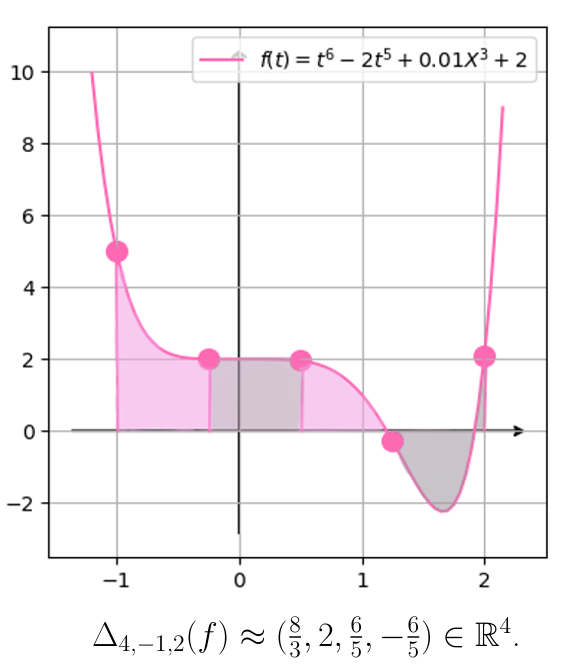
\includegraphics[scale=1.5]{1En_2} 
		\caption{Ejemplo con $n=4$, $a=-1$, $b=2$ y
		$f(t)= t^{6}-2t^{5}+0.01t^{3}+2$}
 	\end{measuredfigure}
 \end{figure}






\noindent
Demostremos que, si escogemos
\begin{itemize}
\item para $0 \leq k \leq n-1$ funciones polinomiales
$g_{k}(t) \in \IR[x]$
\begin{equation}
\label{eq10: 3Nov}
g_{k}(t)= \suma{i=0}{k}{c_{k,i}t^{i}},
\hspace{0.2cm} c_{k, k} >0,
\end{equation}
de grado $k$ y coeficiente principal 
$c_{k,k}$ positivo, 

\item cualquier intervalo $[a,b]$ que partimos 
uniformemente con la malla de $n+1$ puntos
$\cali{P}_{n}= \{ t_{j} \}_{j=0}^{n}$ 
definida en \eqref{eq1: 2En},

\end{itemize}

y si definimos, para toda $0\leq k \leq  n-1$
al vector $u_{k}$ en función de $g_{k}$ como 
\begin{equation}
\label{eq1: 3Nov}
u_{k}:= \Delta_{n,a,b}(g_{k})
= \left( \frac{1}{h} 
\integ{t_{j-1}}{t_{j}}{g_{k}(t)dt} \right)_{j=1}^{n} , 
\end{equation}
entonces los primeros $i$ vectores
de la forma \eqref{eq1: 3Nov}
generan a los espacios $W_{n,i}$
definidos antes en 
\ref{notacion: Pn, fk, Wi, vk},
son linealmente independientes y,
después de ortonormalizarse con 
el proceso de G-S,
obtenemos a los elementos de la base $\cali{L}^{n}$.

Comencemos demostrando la independencia lineal
de los $n$ vectores \eqref{eq1: 3Nov}. Al igual que para
la demostración del resultado análogo 
\ref{Teorema1},
la prueba de este hecho se basa en el teorema
fundamental del álgebra.

\begin{prop}
\label{prop: los uk forman una base de Rn}
Sea $n \in \IN$. El 
subconjunto $\{u_{k} : \hspace{0.1cm} 0 \leq k \leq n-1 \}$
de $\IR^{n}$ , con
$u_{k}$ los $n$ vectores definidos en 
\eqref{eq1: 3Nov},
es linealmente independiente.
\end{prop}
\noindent
\textbf{Demostración.}
Supongamos, por el contrario, 
que existen números reales $a_{k}$, con $0 \leq k \leq n-1$,
no todos cero tales que se tenga la siguiente igualdad en $\IR^{n}$:
\begin{equation}
\label{eq8: 3Nov}
\suma{k=0}{n-1}{a_{k}u_{k}}=0
\end{equation}
Desglosando
la igualdad \eqref{eq8: 3Nov} 
entrada a entrada, descomponemos
a esta en el siguiente sistema de $n$ ecuaciones en $\IR$:
\[
\suma{k=0}{n-1}{ \frac{a_{k}}{h} \int_{t_{j-1}}^{t_{j}}g_{k}(t)\ dt} = 0,
\hspace{0.2cm} 1 \leq j \leq n.
\]
Multiplicando este sistema por $h$, llegamos a las
$n$ igualdades
\begin{equation}
\label{eq2: 2En}
\suma{k=0}{n-1}{a_{k} \int_{t_{j-1}}^{t_{j}}g_{k}(t)\ dt} = 0,
\hspace{0.2cm} 1 \leq j \leq n.
\end{equation}
Por la linealidad de la integral, el sistema \eqref{eq2: 2En}
se reescribe como
\begin{equation}
\label{eq9: 3Nov}
\int_{t_{j-1}}^{t_{j}}p(t)\ dt =0,
\hspace{0.2cm} 1 \leq j \leq n,
\end{equation}


\noindent donde $p$ es el polinomio 
\begin{equation}
\label{eq3: 2En}
p(t):=\suma{k=0}{n-1}{a_{k}g_{k}(t)}. 
\end{equation}
Como todos los polinomios $g_{i}$ son,
por hipótesis, de 
grado menor a $n$ y linealmente independientes
(en el espacio $\IR[x]$),
y se ha supuesto que no
todos los
coeficientes $a_{i}$ son cero, el polinomio
$p$ definido en \eqref{eq3: 2En} es no cero y de grado
menor a $n$. \\

Según el sistema \eqref{eq9: 3Nov}, en cada uno
de los intervalos
\[
I_{j}:=[t_{j-1}, t_{j}], \hspace{0.2cm} 1 \leq j \leq n,
\]

\noindent la función polinomial $p$, continua en todos ellos, 
integra cero. \\

Ahora bien, si en $I_{j}$ la función $p$ fuese siempre
positiva, la integral de esta sería positiva; si fuese
siempre negativa, la integral también
(c.f. \TODO{teorema spivak?}). Existen entonces
puntos $a_{j}$ y $ b_{j}$ en $I_{j}$ tales que
\[
p(a_{j})<0 \hspace{0.2cm} \text{y}
\hspace{0.2cm} p(b_{j})>0.
\]

\noindent Aplicando el teorema del valor intermedio
\TODO{referencia}, 
deducimos la existencia de un 
$r_{j}$ entre $a_{j}$ y 
$b_{j}$ (y que entonces será punto
interior de $I_{j}$) tal que $p(r_{j})=0$;
así, para cada $1 \leq j \leq n$,
hemos
encontrado una raíz $r_{j}$ de $p$ en int($I_{j}$);
por ser ajenos los interiores de los intervalos $I_{j}$,
estamos seguros de que las $n$ raices $r_{j}$ son distintas
entre sí.
Llegamos así
a que el polinomio no cero $p$, cuyo grado es a lo más $n-1$,
tiene al menos $n$ raíces distintas; esto
contradice la proposición \ref{prop: cita TFA}.
\QEDB
\vspace{0.2cm}

\begin{prop}
\label{prop: uk son discretizaciones pol...}
Sean $n \in \IN$. Para toda $0 \leq k\leq n-1$, si
$g_{k} \in \IR[x]$ es como en \eqref{eq10: 3Nov}
y $u_{k} \in \IR^{n}$ como en
\eqref{eq1: 3Nov}, entonces
$u_{k}$ es la discretización en una malla uniforme
de $n$ puntos de un polinomio de grado $k$
y coeficiente principal positivo. En particular,
$u_{k} \in W_{n,k}$.
\end{prop}
\noindent
\textbf{Demostración.}
La $j-$ésima entrada del vector $u_{k}$
(con $1 \leq j \leq n$)
es, según la igualdad \eqref{eq1: 3Nov},

\begin{align} 
\frac{1}{h} \int_{t_{j-1}}^{t_{j}}{g_{k}(t)} \,dt = &
\frac{1}{h} \int_{t_{j-1}}^{t_{j}}{\suma{i=0}{k}{c_{k,i}t^{i}}} \,dt 
\nonumber \\
= & \frac{1}{h} \suma{i=0}{k}{\int_{t_{j-1}}^{t_{j}}{c_{k,i}t^{i}} \, dt}
\nonumber \\
= & \frac{1}{h} \suma{i=0}{k}{
\frac{c_{k,i}}{i+1}t^{i+1} | ^{t=t_{j}}_{t=t_{j-1}}
} 
\nonumber \\
= & \frac{1}{h} \suma{i=0}{k}{
\frac{c_{k,i}}{i+1}t^{i+1} | ^{t=t_{j-1}+\frac{b-a}{n}}_{t=t_{j-1}}} 
\nonumber \\
= & 
\frac{1}{h} \suma{i=0}{k}{
\frac{c_{k,i}}{i+1} \left( t_{j-1}+ \frac{b-a}{n} \right)^{i+1}}-
\frac{1}{h} \suma{i=0}{k}{
\frac{c_{k,i}}{i+1} t_{j-1}^{i+1}}; \nonumber\\
\end{align}
esta última expresión, en principio, es un polinomio
de grado a lo más $k+1$,
que denotaremos por $q_{k}$, evaluado en $t_{j-1}$,
y que está dado por la expresión
\begin{equation} \label{eq2: 5Nov}
q_{k}(t)= \frac{1}{h} \suma{i=0}{k}{
\frac{c_{k,i}}{i+1} \left(t+ \frac{b-a}{n} \right)^{i+1}}-
\frac{1}{h} \suma{i=0}{k}{
\frac{c_{k,i}}{i+1} t^{i+1}}.
\end{equation}

\begin{itemize}
\item Note que las potencias de orden $k+1$ del argumento
$t$ en la expresión \eqref{eq2: 5Nov}
se dan
cuando en la primera y segunda suma el índice $i$
vale $k$; 
tal parte de la suma es 
\begin{equation}
\label{eq1: 5Nov}
\frac{1}{h} \frac{c_{k,k}}{k+1} \left(t+\frac{b-a}{n} \right)^{k+1}-
\frac{1}{h} \frac{c_{k,k}}{k+1} t^{k+1}=
\frac{1}{h} \frac{c_{k,k}}{k+1} t^{k+1}-\frac{1}{h} \frac{c_{k,k}}{k+1} t^{k+1}+ (*)=(*),
\end{equation} 
donde $(*)$ denota un sumando que no contiene potencias de orden
$k+1$ de $t$ (y que, por lo tanto, no interesa para conocer
el coeficiente de $t^{k+1}$).
Así, según \eqref{eq1: 5Nov}, el grado
de $q_{k}$ es a lo más $k$.
\item Busquemos ahora el coeficiente de $q_{k}$ asociado a la
potencia $k$; aparece en
el lado derecho de \eqref{eq2: 5Nov} la potencia $k$
de $t$ cuando en el primer sumando $i=k, k-1$
y también cuando en el segundo sumando $i=k-1$;
así, el coeficiente buscado es
\begin{equation}
\label{eq3: 5Nov}
\frac{1}{h} \frac{c_{k,k}}{k+1}(k+1)\frac{b-a}{n} 
+\frac{1}{h} \frac{c_{k,k-1}}{k}-
\frac{1}{h} \frac{c_{k,k-1}}{k} = 
\frac{1}{h} \frac{c_{k,k}(b-a)}{kn}.
\end{equation}
Puesto que, por hipótesis (c.f. 
condición \eqref{eq10: 3Nov})
el número $c_{k,k}$ es positivo, tenemos que 
el coeficiente principal \ref{eq3: 5Nov}
de $q_{k}$ es positivo.
\end{itemize}


Según todo lo anterior, $u_{k}$
es el polinomio discreto obtenido al evaluar
al polinomio $q_{k}$ (cuyo grado es $k$ y tiene
coeficiente principal \eqref{eq3: 5Nov},
de hecho, es positivo)
en la malla uniforme 
$\cali{P}_{n}=\{t_{j}\}_{j=0}^{n-1}$.
De esto y el teorema 
\ref{cor: propiedades importantes de espacios Wi}
se deduce la pertenecia de $u_{k}$ al espacio $W_{n,k}$.
\QEDB
\vspace{0.2cm}

Recapitulemos; hemos demostrado que 
el subconjunto
\begin{equation}
\label{eq4: 2En}
\{u_{k}: \hspace{0.2cm} 0\leq k \leq n-1 \}
\end{equation}
de $\IR^{n}$
\begin{itemize}
\item es linealmente independiente 
(c.f. proposición \ref{prop: los uk forman una base de Rn}), y que,
\item para toda $0\leq k \leq n-1$, $u_{k}$
es la discretización en una malla uniforme
de $n$ puntos de un polinomio de grado $k$
y coeficiente principal positivo
(c.f. proposición \ref{prop: uk son discretizaciones pol...});
\end{itemize}
así, \eqref{eq4: 2En} es una colección de
polinomios que satisface las condiciones pedidas  
en la subsección
\ref{Generalización que involucra a la discretización Omega n}.
Concluimos, según lo demostrado en esa subsección, 
que el resultado de ortonormalizar la 
base $\{u_{k}\}_{k=0}^{n-1}$ de $\IR^{n}$
(construida, recuerde, a partir del operador de 
discretización $\Delta_{n, a, b}$)
es nuestra base de Legendre
discreta definida en 
\ref{def: base de Legendre discreta}.

\begin{figure}[H]
\centering\captionsetup{format = hang}
	\begin{measuredfigure}
		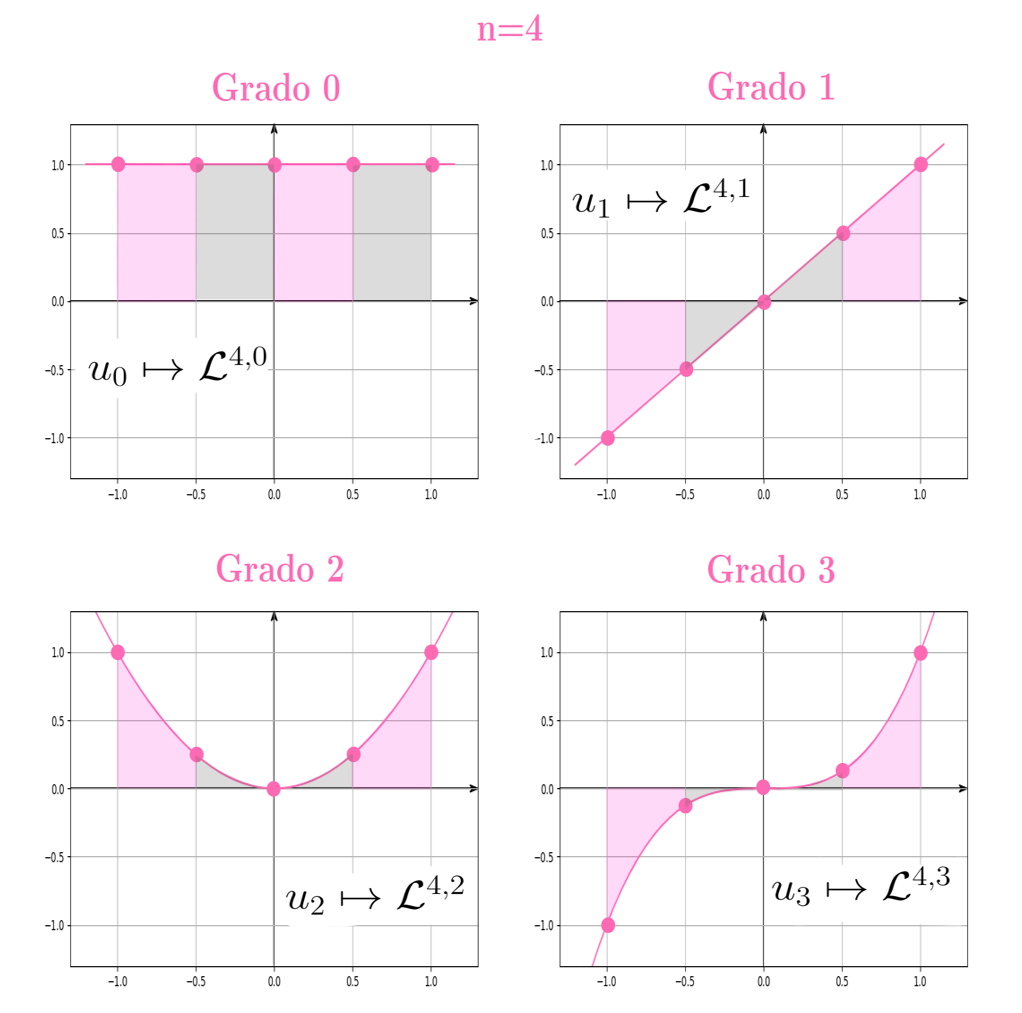
\includegraphics[scale=0.4]{5Dic_1} 
	\caption{Al comenzar este
	trabajo de tesis,
	nuestra definición original de la base $\cali{L}^{n}$
	consistía en discretizar a los polinomios
	$f_{k}$, $0 \leq k \leq n-1$ con el operador $\Delta_{n,-1,1}$.
	En la figura se ilustra este proceso para cuando $n=4$.}
 	\end{measuredfigure}
 \end{figure}
        
     
    
    
\begin{figure}[H]
\centering\captionsetup{format = hang}
	\begin{measuredfigure}
		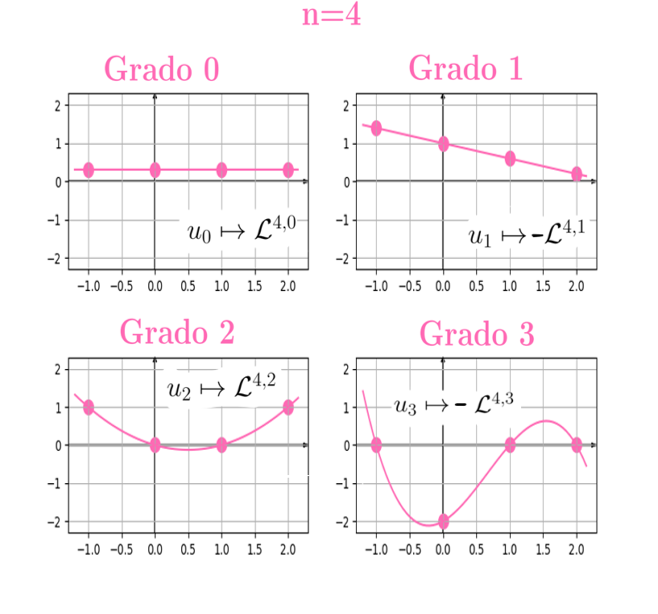
\includegraphics[scale=0.71]{5Dic_2} 
		\caption{Según la teoría
		 desarrollada en esta sección, 
		 fijada una dimensión $n$, podemos
	cambiar tanto la malla uniforme como el método 
	de discretización; después
	de ortonormalizar, salvo por cambios de signo,
	obtendremos a la
	base $\cali{L}^{n}$. 
	Es el coeficiente principal del polinomio
	discretizado para obtener al vector $v_{k}$ 
	el que determina
	el signo correcto. Para el ejemplo mostrado
	en la imagen (donde se ha fijado $n=4$), se
	han considerado a los polinomios
	$h_{0}(t)=0.3$, $h_{1}(t)=-0.4t+1$,
	$h_{2}(t)=0.25t^{2}-0.5t$ y $h_{3}(t)=-t^{3}+2t^{2}+t-2$.
	Como se destaca, los polinomios con coeficiente principal
	negativo (en este caso, los de grados $1$ y $3$)
	dan lugar a los respectivos polinomios de Legendre
	discretos con signo negativo.}
 	\end{measuredfigure}
 \end{figure}
 